%% ========================================================================
%%								Fabian Pribahsnik
%% ========================================================================
%%
%% ========================================================================
%%%% Basic settings
%% ========================================================================

%%%%%%%%%%	used in style.tex	%%%%%%%%%%
\newcommand{\myfontsize}{12pt}
%% e.g., 10pt, 11pt, 12pt
%% The font size of the main text in pt (points).

\newcommand{\mypapersize}{A4}
%% e.g., "A4", "letter", "legal", "executive", ...
%% The size of the paper of the resulting PDF file.

\newcommand{\myparskip}{half}
%% e.g., "no", "full", "half", ...
%% How to separate paragraphs: indention ("no") or spacing ("half", "full", ...).

\newcommand{\mydraft}{false}
%% "true" or "false"
%% Use of draft mode: If true, included graphics are replaced by empty rectangles (of same size) and overfull boxes 
%% (in margin space) are marked with black box (-> easy to spot!)

\newcommand{\myBCOR}{0mm}
%% Inner binding correction. This value depends on the method which is being used to bind your printed result. Some
%% techniques do not require a binding correction at all ("0mm"), other require for example "5mm". Refer to KOMA
%% script documentation for a detailed explanation what a binding correction is and how to measure it.                                         

\newcommand{\mylaterality}{twoside}
%% "oneside" or "twoside"
%% Either you are creating a document which is printed on both, left pages and right pages (twoside) or you create a
%% document which is printed on right pages only (oneside).

\newcommand{\mybiblatexstyle}{numeric}
%% e.g., "alphabetic", "authoryear", ...
%% The biblatex style which is being used for referencing. See biblatex documentation for further details and more values.

\newcommand{\mybiblatexbackref}{true} 
%% "true" or "false"
%% If true: create backward links from reference to citations.

\newcommand{\mybiblatexfile}{references.bib}
%% Name of the biblatex file that holds the references.

\newcommand{\mytodonotesoptions}{}
%% e.g., "" (empty), "disable", ...
%% Options for the todonotes-package. If "disable", all todonotes will be hidden (including listoftodos).




%% ========================================================================
%%								Fabian Pribahsnik
%% ========================================================================
%%
%% ========================================================================
%%						All different kinds of style settings and other stuff
%% ========================================================================

\documentclass[% KOMA Script
fontsize=\myfontsize,%% size of the main text
paper=\mypapersize,  %% paper format
parskip=\myparskip,  %% vertical space between paragraphs (instead of indenting first par-line)
DIV=calc,            %% calculates a good DIV value for type area; 66 characters/line is great
%headinclude=true,    %% is header part of margin space or part of page content?
headinclude=false,
footinclude=false,   %% is footer part of margin space or part of page content?
open=right,          %% "right" or "left": start new chapter on right or left page
appendixprefix=true, %% adds appendix prefix; only for book-classes with \backmatter
bibliography=totoc,  %% adds the bibliography to table of contents (without number)
draft=\mydraft,      %% if true: included graphics are omitted and black boxes
                     %%          mark overfull boxes in margin space
%BCOR=\myBCOR,        %% binding correction (depends on how you bind
                     %% the resulting printout.
\mylaterality        %% oneside: document is not printed on left and right sides, only right side
                     %% twoside: document is printed on left and right sides
]{scrbook}  %% article class of KOMA: "scrartcl", "scrreprt", or "scrbook".
            %% CAUTION: If documentclass will be changed, *many* other things
            %%          change as well like heading structure, ...
            
\usepackage[utf8]{inputenc} %% UTF8 as input characters
\usepackage[ngerman,american]{babel}  %% used languages; default language is *last* language of options
\usepackage{csquotes}	%% quotations
\usepackage{scrpage2} %%  advanced page style using KOMA
\usepackage{graphicx}
%\usepackage[pdftex]{graphicx}%% The widely used package to use graphical images within a \LaTeX{} document.
\usepackage[\mytodonotesoptions]{todonotes}  %% option "disable" removes all todonotes output from resulting document
\usepackage{enumitem} %% enables the user to customize the enumerate,.. (make lists with a), b), c) or A), B), ....)
\usepackage{amsmath} %% math environment for equations
\usepackage{amsthm}   %% math environment for theorems, definitions,...
\usepackage{amssymb} %% blackboard bold symbols for expectation,...
\usepackage{algorithm} % environment to write pseudo code 
\usepackage[noend]{algpseudocode}% environment to write pseudo code 
\usepackage{xifthen}    %% makes it possible to make the output of a new command dependent on the input values for that command. (see articlequote)
\usepackage{tabu, booktabs, makecell} %%tabu: make tables within the text; booktabs: vertical lines; makecell: multiline cells
\usepackage[labelfont=bf]{caption}%%needed to reference on tables and figures make Table,... bold
\usepackage{actuarialangle} %%needed for the annuity-symbol
\usepackage{eurosym} %% get the euro symbol
\usepackage{pdflscape} %% rotate pages to landscape (e.g. big tables)
\usepackage{afterpage} %% clear all floating objects (used for pdflscape)
\usepackage{enumitem} %% for roman enumeration
\usepackage{bbm} %% make the math symbol for Indicator 1 (\mathbbm{1})
\usepackage{listings} %% implemnt R code 
\usepackage{multicol} %% itemize in multiple columns. 
\usepackage{tikz} %% draw in latex
\usetikzlibrary{matrix,chains,positioning,decorations.pathreplacing,arrows, backgrounds}
\usetikzlibrary{positioning,calc}


\usepackage[backend=biber, %% using "biber" to compile references (instead of "biblatex")
style=\mybiblatexstyle, %% see biblatex documentation
%dashed=\mybiblatexdashed, %% do *not* replace recurring reference authors with a dash
backref=\mybiblatexbackref, %% create backlings from references to citations
natbib=true, %% offering natbib-compatible commands
hyperref=true, %% using hyperref-package references
]{biblatex}  %% remove, if using BibTeX instead of biblatex

\addbibresource{\mybiblatexfile}			%% Name of the biblatex file that holds the references.

%define colours
\definecolor{backcolour}{rgb}{0.95,0.95,0.92}
\definecolor{codepurple}{rgb}{0.58,0,0.82}

\lstset{%Settings for how I want the code included
	language=R,
	basicstyle=\scriptsize\ttfamily,
	commentstyle=\ttfamily\color{blue},
	stringstyle=\color{codepurple},
	keywordstyle=\color{magenta},
	stepnumber=1,
	numbersep=5pt,
	backgroundcolor=\color{backcolour},
	showspaces=false,
	showstringspaces=false,
	showtabs=false,
	numbers=left,
	frame=single,
	tabsize=2,
	captionpos=b,
	breaklines=true,
	breakatwhitespace=false,
	escapeinside={},
	morekeywords={NULL},
	otherkeywords={\%*\%, \%\%}, % make %*% (matrix-multiplication) be highlighted
	deletekeywords={fitted, resid, R}
}
%% ========================================================================
%%							mycommands
%% ========================================================================

\newcommand{\articlequote}[3]{
	\begin{quotation}
		\begin{center}
			\textit{#1}
			% \ifthenelse{〈test expression〉}{〈true code〉}{〈false code〉}
			% \equal{〈string1〉}{〈string2〉}
			\ifthenelse{\equal{#2}{}}{}{\\ \medskip \textbf{#2}}
			\bigskip
		\end{center}
	#3
	\end{quotation}
}

\newcommand{\E}{\mathbb{E}}
\newcommand{\R}{\mathbb{R}}
\newcommand{\N}{\mathbb{N}}
\newcommand{\V}{\mathcal{V}}


% define new maths operators 
\DeclareMathOperator*{\argmin}{arg\,min} % thin space, limits underneath in displays

% used for enumeration styles
\newcommand{\subscript}[2]{$#1 _ #2$}

% environments for definition, theorems, remarks,...
\newtheorem{definition}{Definition}[chapter]
\newtheorem{corollary}{Corollary}[chapter]
\newtheorem{theorem}{Theorem}[chapter]
\newtheorem{lemma}{Lemma}[chapter]
\newtheorem{example}{Example}[chapter]
\newtheorem{remark}{Remark}[chapter]

% draw right angle with tikz
\newcommand*{\rightangle}[3]{% #1 = point, #2 = start angle, #3 = radius
	\draw[shift={(#2:#3)}] (#1) arc[start angle=#2, delta angle=90, radius = #3];
	\fill[shift={(#2+45:#3/2)}] (#1) circle[radius=1.25\pgflinewidth];
}

\newcommand{\textfield}[2]{
	\vbox{
		\hsize=#1\kern3cm\hrule\kern1ex
		\hbox to \hsize{\strut\hfil\footnotesize#2\hfil}
	}
}

\newcommand*{\estimates}{\mathrel{\widehat=}}

\newcommand{\norm}[1]{\left\lVert#1\right\rVert}

% make the everything dependent --> 1 counter for all 
	%\newtheorem{corollary}[definition]{Corollary}
	%\newtheorem{lemma}[definition]{Lemma}
	%\newtheorem{example}[definition]{Example}




%\newwatermark*[allpages,color=red!50,angle=45,scale=3,xpos=0,ypos=0]{DRAFT}


%% ========================================================================
%%%% begin{document}
%% ========================================================================

\begin{document}

\frontmatter                    				%% KOMA: roman page numbers and such; only available in scrbook
%% ========================================================================
%%%% 						Fabian Pribahsnik
%% ========================================================================


\begin{titlepage}

{\sffamily

\begin{center}


\includegraphics[width=30mm]{figures/TU_Logo}

\vfill\vfill\vfill
\vfill\vfill\vfill

Fabian Peter Pribahsnik, BSc.

\vfill\vfill\vfill

{\LARGE\bfseries Let the data tell us their story \\ Machine learning with insurance policies}


\vfill\vfill\vfill
\vfill\vfill\vfill


{\bfseries\large Master's Thesis}

to achieve the university degree of

Master of Science

Financial and Actuarial Mathematics


\vfill\vfill\vfill


submitted to

\vfill

{\bfseries\large Vienna University of Technology}

Institute of Statistics and Mathematical Methods in Economics


\vfill\vfill\vfill


Supervisor

Univ.Prof. Dipl.-Math. Dr.rer.nat. Thorsten  Rheinländer
%usually not mentioned on titlepage:% Evaluator: \myevaluator

\vfill

\hbox to \hsize{\textfield{3cm}{Date}\hfil\textfield{4cm}{Supervisor}\hfil\textfield{4cm}{Author}}

\end{center}
}%% end sffamily
\end{titlepage}

\newpage
            		%% include title page
\cleardoublepage					%% starts next text on an odd page 
%% ========================================================================
%%%% 					Fabian Pribahsnik
%% ========================================================================


\section*{Affidavit}
I declare that I have authored this thesis independently, that I have
not used other than the declared sources/resources, and that I have
explicitly indicated all material which has been quoted either
literally or by content from the sources used. 

\hbox to \hsize{\textfield{4cm}{Date}\hfil\hfil\textfield{7cm}{Fabian Pribahsnik}}
				%% include the affidavit
\cleardoublepage					%% starts next text on an odd page 
%% include the abstract without chapter number but include it on table of contents:
\addcontentsline{toc}{chapter}{Abstract}	
%% ========================================================================
%%							Abstract
%% ========================================================================


\chapter*{Abstract}
\label{cha:abstract}


Insurance companies are facing a huge amount of regulations, including various guidelines addressing forecast scenario calculations for the policies in the portfolio. Taking the hundreds of thousands policies into account an average insurance company has in its portfolio on can easily see that these scenario calculations are very time consuming. Due to the rising number of policies and the very tight time schedule introduced with Solvency II insurance companies are looking for ways to reduce the computational time significantly. In the past years different approaches were developed and already used for grouping similar policies together and therefore reducing the computation time. The currently used algorithms are ranging from just grouping policies with exactly the same attributes together to basic cluster algorithms like k-means. This work highlights potential problems with the algorithms currently used and tries to implement some machine learning techniques to accomplish the task of grouping. 
					%% inlcude abstract

\tableofcontents					%% inlcude table of contents
\listoffigures						%% inlcude table of figures

\listoftodos						%% include the list of to-dos
	
\mainmatter                     %% KOMA: marks main part using arabic page numbers and such; only available in scrbook

%% ========================================================================
%%							Introduction
%% ========================================================================


\chapter{Introduction}
\label{cha:introduction}

A fundamental problem faced by many insurance companies is the projection of the insurance portfolio into the future. In a projection, the future cash flows for each individual policy must be calculated on the basis of actuarial principles and then saved for further analysis. Depending on the purpose of the forecast, these cash flows have to be provided either on a monthly or annually basis.Together with the contractually agreed benefits to the policyholder, a wide variety of other parameters must also be taken into account and modelled in such projections. These include, for example, all contract changes that may occur during the duration of the contract, such as a premium pause, a surrender or the occurrence of a claim. While the calculation of a small set of policies over a relatively short time horizon does not pose a challenge in terms of computation time, this fact changes greatly when projecting entire portfolios. This problem is particularly severe for life insurance portfolios. These contracts often have durations of several decades and the portfolios tend to grow over time as fewer policyholders leave than new ones are added. Even with the optimistic assumption that the complete projection of a single contract only takes a hundredth of a second, the computing time adds up to several hours for a portfolio with several million policies. As the liabilities are projected over a period of several decades, it is also essential to simulate the development of the assets, underlying the liabilities, over this period. Even under the assumption that the assets can be represented by a small number of different types of investments, their projection additionally increases the run time of the projection. The simultaneous simulation of the asset and liability portfolios results in further factors that have to be taken into account with respect to the behaviour of policyholders during the contract term. If one assumes that the policyholder behaviour during the projection period also depends on external parameters such as the current interest rates on savings, one also has to include that effect into the simulation. This finally results in a dynamic interaction of all components which can be summarized in a simplified pseudo code given in algorithm \ref{alg:interaction}:

\begin{algorithm}
	\caption{Simplified dynamic interaction scheme of portfolio projection}\label{alg:interaction}
	\begin{algorithmic}
		\\
		\begin{enumerate}
			\item Initialisation of assets and liabilities at time $t = 0$.
			\item  Iteration till the end of the projection horizon is reached:
			\begin{enumerate}[label=\emph{\alph*})]
				\item Calculation of one time step for the liabilities. This means that all policies are projected to the next year ($t \mapsto t+1$). 
				\item Calculation of one time step for the assets. This means that the returns of all investments are simulated for the next year.
				\item Simulation of the dynamic policyholder behaviour based on the current economic parameters from the previous step.
				\item Application of pre-defined management decisions based on current developments in assets and liabilities. This means that in this step it is determined how high the dividend per share, for example, will be for this year. 
			\end{enumerate}
		\end{enumerate}
	\end{algorithmic}
\end{algorithm}

Note that during an iteration (algorithm \ref{alg:interaction}, 2a - 2d ) all results must be kept in memory until every decision for that loop is made and the next iteration starts. Assuming that there is a portfolio of several million policies and for each policy at least a few dozen variables are relevant for the decision making process, a memory requirement of at least hundreds of million individual values emerges. Also the simulations of the assets side and the subsequent management decisions have a considerable memory requirement. All this leads to the fact that the projection models currently used in the insurance industry are extremely demanding in terms of their memory requirements and execution time. There are at least two different ways to address this problem:

\begin{itemize}
	\item Outsourcing of calculations to an external high performance infrastructure.
	\item Data compression in the sense that similar policies are grouped together and only the grouped portfolio is calculated.
\end{itemize}

With the increasing availability of cloud services, it is already an option these days to outsource complex computing operations to specialized providers. It is possible to rent different types of computing capacities for a certain period of time without much effort and run the projections there. The big advantage of this option is that there is no need to set up, maintain and configure an infrastructure. Since personal data such as age or gender are always used in the projection of insurance contracts, potential problems could arise with respect to the General Data Protection Regulation \cite{datenschutz}. Many companies have therefore decided to compress the insurance portfolio and therefore reducing the memory requirements using various techniques. It is then feasible to calculate the projections with infrastructure that is owned by the company. This approach has the big advantage that it avoids possible problems with data protection issues and also reduces the dependency on external services. On the other hand, an additional effort has to be made to compress the portfolio in a proper way. Of course, it is of utmost importance that the compressed portfolio has the same characteristics and produces the same cash flows as the non-compressed one. Exactly here, this thesis kicks in and shows possible ways, how a portfolio of insurance contracts can be compressed. 

%--------------------------------------------------------------------- Problem formulation -----------------------------------------------------------------------
\section{Problem formulation}
For the sake of simplicity all values calculated by the projection tool are referred to as cash flows regardless of whether they are non-cumulative values such as the reserve or actual cash flows such as the premium. The task is to find a portfolio with a reduced number of policies, the so called grouped portfolio, so that the projected cash flows match those from the reference  portfolio as accurately as possible. In order to be able to define what accurately means in terms of cash flow deviations, some basic concepts must be defined first . 

\begin{definition}
	Let $\V$ = \{V, V is a valid insurance contract\} be the set of all valid insurance contracts. A finite set of elements $P \subset \V$ is called a portfolio and the number of policies within that portfolio is determined by its cardinality.
\end{definition}

\begin{definition}
	Let $P \subset \V$ be a portfolio of n policies (i.e. $\vert P \vert$ = n) and $m$ the number of projected cash flows by the simulation $s$. Then the individual cash flows corresponding to $P$ are encoded in $A \in \R^{m \times n}$ and the summed cash flows are encoded in $b \in \R^m$.

	\begin{equation*}
	\begin{aligned}[c]
	s: \V &\rightarrow R^{m \times n}\\
		P & \mapsto s(P)=A\\
	\end{aligned}
	\qquad \qquad
	\begin{aligned}[c]
	s: \V &\rightarrow R^m\\
		P & \mapsto A \cdot \mathbbm{1}_{n \times 1} = b \\
	\end{aligned}
	\end{equation*}
	
\end{definition}

\begin{remark}
	It should be noted that the definition of portfolio is ambiguous. It can include anything from a single policy to all policies held by an insurance company. The usual segmentation into portfolios is often based on the following characteristics:
	\begin{itemize}
		\item All contracts of a singe tariff are put into one portfolio.
		\item All contracts of a tariff group (endowment insurances, pension insurances,...) are put into one portfolio. 
		\item All contracts sold in the same country are put into one portfolio.
	\end{itemize} 
\end{remark}

\begin{example}
	Let $P \subset \V$ be a portfolio with $\vert P \vert$ = 1000, the number of cash flows $m = 180$. Then the cash flows generated by the projection software can be described as:
	
	\begin{equation*}
	\begin{aligned}[c]	
		A= 
		\left( 
			\begin{array}{cccc}
				a_{1,1} 	& a_{1,2} 	& \cdots 	& a_{1,1000} \\
				a_{2,1} 	& \ddots	&  			& a_{2,1000} \\
				\vdots 		&  			& \ddots 	& \vdots \\
				a_{180,1} 	& a_{180,2}	& \cdots 	& a_{180,1000} \\
			\end{array}
		\right)	
	\end{aligned}
	\qquad
	\begin{aligned}[c]
		b = 
		\left( 
			\begin{array}{c}
			b_{1} \\
			b_{2}\\
			\vdots\\
			b_{180}\\
			\end{array}
		\right)	
		=
		\left( 
			\begin{array}{c}
			\sum_{i = 1}^{1000} a_{1,i} \\
			\sum_{i = 1}^{1000} a_{2,i}\\
			\vdots\\
			\sum_{i = 1}^{1000} a_{180,i}\\
			\end{array}
		\right)	
	\end{aligned}	
	\end{equation*}
\end{example}

A column in matrix $A$ describes all cash flows generated by this policy. One row of matrix $A$ describes the same cash flow generated by the different policies. By calculating line totals, the corresponding cash flow is obtained at portfolio level. The individual policy by policy cash flows are therefore given in matrix $A$, and the portfolio cash flows in vector $b$. 

\begin{definition}
	Let $P \subset \V$ be a portfolio with $\vert P \vert = n$, $\tilde{P} \subset \V$  the grouped portfolio with $\vert \tilde{P} \vert = \tilde{n}$, $\tilde{n} < n$ and $w \in \R^m_{\geq 0} = \{x \in \R^m, x \geq 0\}$ a vector of weights. Then the weighted sum of squares of the cash flows over the entire projection horizon between the grouped portfolio $\tilde{P}$ and the ungrouped one $P$ is given by: 
	
	\begin{equation}\label{eq:objective_function}
		WSS_{total} = \lVert w \circ (b - \tilde{b})\lVert_2^2
	\end{equation}
\end{definition}

The weighting parameter $w$ makes it possible to make deviations from certain cash flows more or less important by weighting them differently. This can be useful, for example, to weight deviations at the end of the projection period less heavily compared to deviations at the beginning of the projection horizon. Particularly with projection horizons of 30 years and more, it may make sense to weight deviations in cash flows less strongly at a later point in time. 

\begin{remark}
	In a situation where every deviation of cash flows between the grouped and the ungrouped portfolio is equally important, the elements of $w$ are all one. In this situation equation (\ref{eq:objective_function}) simplifies to:	
	\begin{equation}\label{eq:objective_function_simple}
		WSS_{total} = \lVert b - \tilde{b}\lVert_2^2
	\end{equation}	
\end{remark}

The aim is to develop a method which is capable of finding a suitable grouped portfolio for each portfolio at hand so that (\ref{eq:objective_function}) is sufficiently small. If there are several methods that come to similar results, then of course the one that needs the smallest grouped portfolio (i.e. smallest $\tilde{n}$) to generate the desired cash flows is of interest. 


This thesis reviews the currently used technique for grouping policies together and introduces furthermore some new approaches on how life insurance policies can be grouped together. We will therefore highlight drawbacks and advantages with a special emphasis on the regulatory requirements of every approach discussed. Theoretical considerations as well as practical implementations and tests with real world data will provide us some information on which method an insurance company should work with in order to obtain the best grouping results.  

This thesis is structured as follows: First we give an overview on the legal framework which lays down the minimum requirements for grouping-approaches in insurance companies and introduce the two types of statistical learning, namely supervised and unsupervised. We then discuss how sensitive main characteristics of a policy are with respect to the interest rate, the age or the duration to get a better understanding on which parameters are important for grouping purposes. We therefore make a sensitivity analysis with real world data and a widely used projection tool . In the next chapter we introduce the currently used unsupervised learning algorithm k-means and derive some theoretical findings. 
\todo{Weitere Details für jedes Kapitel folgen.}


%--------------------------------------------------------------------- Legal Framework -----------------------------------------------------------------------
\section{Legal Framework}

Solvency II - entered into force on 1 January 2016 - is the European framework for a common insurance supervision. It is intended to achieve a harmonization of the European insurance sector and was implemented in accordance with the Lamfalussy architecture which works on a 4 level basis \cite{Lamfalussy_homepage}. The most significant elements and aims of the new regulation framework can be studied on the homepage of the financial market authority (FMA) \cite{FMA_homepage} and on the homepage of the  European Insurance and Occupational Pensions Authority (EIOPA) \cite{EIOPA_homepage}. This work is intended not to cover all aspects and aims of the new Solvency II regulation framework but focuses on the topic of data quality regarding to the actuarial function. In order to meet all the requirements imposed by Solvency II, insurance companies need to process large amounts of data within a short period. One critical aspect of these calculations is the projection horizon which however should cover the full lifetime of all obligations as stated in \cite{Time_horizon}:
\articlequote{3.83.}{}{The projection horizon used in the calculation of best estimate should
cover the full lifetime of all obligations related to existing insurance and
reinsurance contracts on the date of the valuation.}
\articlequote{3.84.}{}{The determination of the lifetime of insurance and reinsurance obligations shall be based on up-to-date and credible information and realistic assumptions about when the existing insurance and reinsurance obligations will be discharged or cancelled or expired.}
Another aspect needed to be considered is the fact that cash flow calculations need to be done for a variety of different economic scenarios which yields to an enormous computational effort. Due to the tight time schedule, insurance companies are looking for new possibilities to speed up these time consuming calculations. One approach is not to make all these calculations on a per policy level, but on a grouped level where similar policies are grouped together and represented by only a few policies. This approach raises the question of how to maintain data quality as mentioned in the level 1 directive \cite{Directive} while reducing the number of policies.

\articlequote{Article 82}{Data quality and application of approximations, including
case-by-case approaches, for technical provisions}{Member States shall ensure that insurance and reinsurance undertakings
have internal processes and procedures in place to ensure the appropriateness, completeness and accuracy of the data used in the calculation of their technical provisions...}

By publishing the level 2 regulations, supplementing the level 1 directive \cite{Directive} the European Commission is getting more specific on data quality (Article 19 in \cite{Regulations}) and also formulates concrete requirements for grouped policies \cite{Regulations}.

\articlequote{Article 35}{Homogeneous risk groups of life insurance obligations}{The cash flow projections used in the calculation of best estimates for life insurance obligations shall be made separately for each policy. Where the separate calculation for each policy would be an undue burden on the insurance or reinsurance undertaking, it may carry out the projection by grouping policies, provided that the grouping complies with all of the following requirements:
\begin{enumerate}[label=\emph{\alph*})]
\item there are no significant differences in the nature and complexity of the risks underlying the policies that belong to the same group;
\item the grouping of policies does not misrepresent the risk underlying the policies and does not misstate their expenses;
\item the grouping of policies is likely to give approximately the same results for the best estimate calculation as a calculation on a per policy basis, in particular in relation to financial guarantees and contractual options included in the policies.
\end{enumerate} }

These level 2 regulations are a reference point on what to consider when grouping policies together and they are even further specified in the level 3 guidelines issued by EIOPA\cite{Guidelines_TP}. Further details on the level 3 guidelines including feedback statements to the consultation paper (EIOPACP-14/036) and the guidelines can be obtained from \cite{Final_Report}.

%--------------------------------------------------------------------- Statistical Learning -----------------------------------------------------------------------

\section{Statistical Learning}

Statistical learning refers to a set of methods which deals with predicting outcomes based on input variables or finding patterns in data sets. In order to accomplish the task of grouping together similar policies, different approaches from statistical learning can be applied. All these methods can be classified either as supervised or unsupervised. Within the framework of supervised methods, statistical models try to predict output variables $y_i$ based on some input variables $x_i$ where the relation $y=f(x)$ is unknown. It is therefore indispensable to have input as well as output data to parameterize such a model in order to find a prediction $\hat f$ of $f$. Unsupervised methods, in contrast, are used when inputs $x_i$ but no corresponding outputs $y_i$ are available. These methods then try to find some hidden patterns within to data. The task of grouping insurance policies involves many different aspects. On the one hand we have all data needed to apply supervised methods, but on the other hand we are only interested in the patterns that can be revealed by an unsupervised method. The input variables are given by the characteristics of each policy and the corresponding output variables are determined by the projection tool. Our primary goal is not to get a good $\hat f$ because the projection tool, which stands for $f$, is already known. We are more interested in hidden patterns that can be used for grouping purposes. In a first step we will apply unsupervised methods to the data and try to group the policies based on their characteristics and their cash flows. In a further step we will try to use the additional information of $f$ to improve the grouping results if possible. 

					%% inlcude introduction
%% ========================================================================
%%							Sensitivities
%% ========================================================================


\chapter{Sensitivities}
\label{cha:sensitivities}

Grouping together single policies and representing them by just a few representative ones always comes along with a loss of information. A natural question which arises when grouping insurance contracts together is how to determine the main characteristics of the new representative policy. Some characteristics should for technical reasons be defined as the sum of the individual ones, like the sum insured, the premium or the accumulated reserve. This is needed to guarantee the equality between the ungrouped and the grouped portfolio in terms of these characteristics at the beginning of the projection horizon. For other characteristics like the age, the duration or the gender it is not intuitively clear how they should be defined for a representative policy. Possible solutions which can be implemented easily range from taking the weighted average over the value with the highest relative frequency or to just taking the median of the grouped policies. Another difficulty which arises when grouping together policies from different product generations is, how the technical interest rate of the representative contract should be defined. Even if the policies are identical in terms of age, sex, sum insured, duration, costs,... and just differ on their issue date the huge possible differences with respect to the technical interest rate as shown in table \ref{tab:interest_rates} can have enormous impacts on the projected cash flows. 
Already a relative small difference in the technical interest of only one percent causes double digit differences in the guaranteed capital after 1 decade. 

\begin{minipage}{\linewidth}
	\centering
	\begin{tabular}{*{9}{c}}
	\toprule
	\makecell{31.12.\\1994} & \makecell{30.06.\\2000} & \makecell{31.12.\\2003} & \makecell{31.12.\\2005} & 				\makecell{31.03.\\2011}  & \makecell{20.12.\\2012} & \makecell{31.12.\\2014} & \makecell{31.12.\\2015} & 				\makecell{31.12.\\2016}\\
	\midrule
	4\% & 3.25\% & 2.75\% & 2.25\% & 2\% & 1.75\% & 1.5\% & 1\% & 0.5\% \\
	\bottomrule
	\end{tabular}
	\captionof{table}{ Maximum technical interest rates for life insurance contracts issued after the given dates. (see \cite{fakten_trends})}
	\label{tab:interest_rates}
\end{minipage}

It is therefore important to know how sensitive the different output variables of interest which are calculated by the projection tool react if various input parameters are changed slightly. The most basic task is to determine whether the correlation between the input and output variables is positive or negative. There are many output variables which are important for determining if a grouping process has been successful in terms of accuracy or not, but in the subsequent we will focus only on a few of them, namely the premium, the present value of future profits at time 0, the reserve and the yearly claims. Due to the big variety of different insurance products we will just give some general guidelines based on the most important input variables. Most of the life insurance contracts can be built up by the following elementary insurance types and some additional factors for different types of costs. \footnote{For detailed definitions and explanations see \cite{Gerber}.}:
\begin{alignat}{2}
\label{equ:whole_life}
A_x &=\sum_{k=0}^{\infty}v^{k+1} {}_{k}p_x q_{x+k} \quad \quad \quad &&\text{(Whole life insurance)}\\
A_{x:\actuarialangle{n}}^1 &=\sum_{k=0}^{n-1}v^{k+1} {}_{k}p_x q_{x+k} \quad \quad \quad  &&\text{(Term insurance)}\\
A_{x:\actuarialangle{n}} &=\sum_{k=0}^{n-1}v^{k+1} {}_{k}p_x q_{x+k} + v^n{}_{n}p_x\quad \quad &&\text{(Endowment)} \\
\ddot{a}_x &= \sum_{k=0}^{\infty} v^k {}_{k}p_x \quad &&\text{(Whole life annuity)} \\
\label{equ:temp_annuity}
\ddot{a}_{x:\actuarialangle{n}} &= \sum_{k=0}^{n-1} \ddot{a}_{\actuarialangle{k+1}} {}_{k}p_x q_{x+k} + \ddot{a}_{\actuarialangle{n}}~{}_{n}p_x  \quad &&\text{(Temporary life annuity)}
\end{alignat}
These basic types already show that the main characteristics which should be taken care of, when it comes to a grouping process are the age $x$, the duration $n$ and the technical interest rate which is implicitly given by $v$.  The following graphs and analyses are based on an endowment policy with a duration of 25 years, a sum insured of \EUR{10.000} and an investment return of 3\% p.a. over the whole projection horizon. The duration of 25 years is in all subsequent considerations equal to the duration of the premium payments which are made on a yearly basis. All other parameters especially the lapse, paid-up and surrender rates as well as first and second order assumptions can't be given here in detail. 

\section{Age}
\label{sec:age} 
The age of an insured person is one of the main factors which drives the projected outcome because it directly influences the probability of death and survival as shown in (\ref{equ:whole_life}) - (\ref{equ:temp_annuity}). When the age is changed from $x$ to $x+1$ the survival- and death-probabilities ${}_{k}p_x$ and ${}_{k}q_x$ change as well. It is impossible to predict in general whether the probabilities will rise or fall.
\begin{figure}
	\centering
	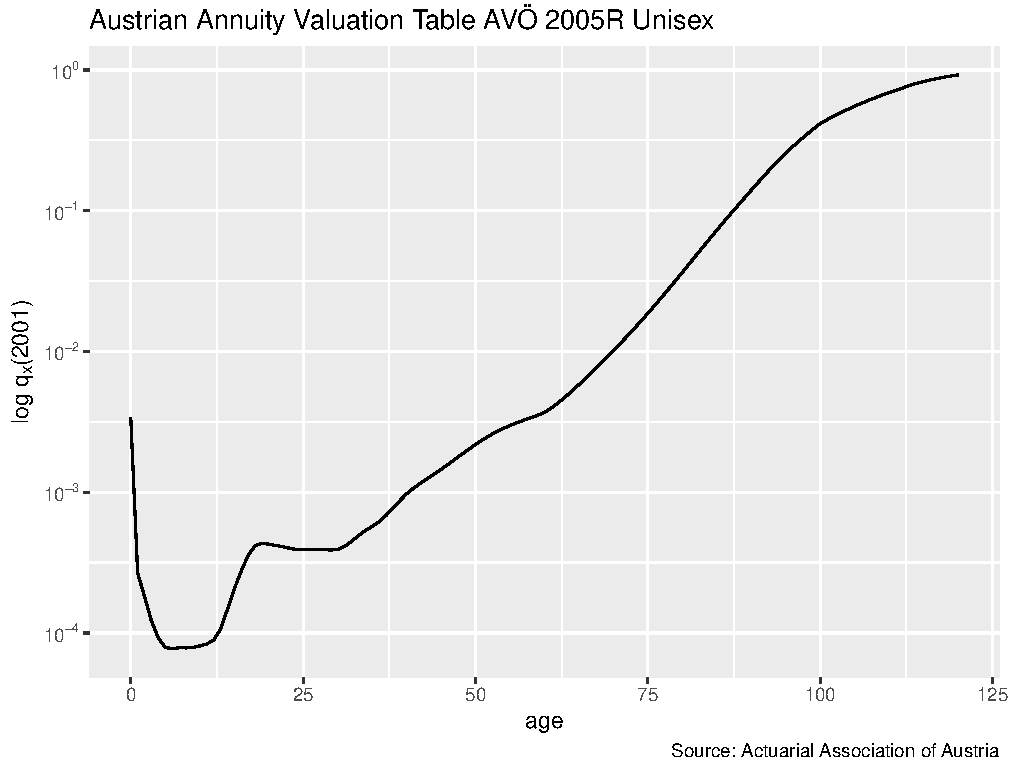
\includegraphics[width=0.9\textwidth]{figures/chapter_sensitivities/Austrian_Annuity_Valuation_Table/avoe_2005R_unisex}
	\caption{Logarithm of the yearly mortality defined by the Austrian Annuity Valuation Table AVÖ 2005R Unisex.}
	\label{fig:sensitivity_annuity_table_graph}
\end{figure}
Figure (\ref{fig:sensitivity_annuity_table_graph}) shows, for example, the graph of logarithmic mortality rates based on the values of the unisex mortality table from the Actuarial Association of Austria \cite{kainhofer2006new}. A high level of non-linearity can be observed, which naturally leads to greater challenges in the grouping.

As known from life tables it is a bit more likely to die just after birth than a bit afterwards and the same is true for people aged around 20.  The exact ages where the probability of survival increases and the probability of death decreases when a person gets a year older depends heavily on the life table and the sex of the insured person. Whether the values for (\ref{equ:whole_life}) - (\ref{equ:temp_annuity}) will rise or fall when the age $x$ is increased by 1 year will therefore depend on $n$, $x$ and the sex of the insured person. To get a better insight into the portfolio, simulation runs for various parameters should be done. 
In figure (\ref{fig:sensitivity_age_claims}) the development of the yearly total claims is plotted against the duration of 25 years. The claims are the amount of money that must be paid to the policyholder at the time of an insured event multiplied by the probability that such an event will occur. Such events can be of all kinds, but the most common are, for example, the death of the insured person or a surrender of the contract. 

For a clearer chart the last cash flow which is the sum insured and therefore substantially larger than the yearly claims is omitted. We see that for younger people (green and red lines) the claims are almost identical in the first years and only deviate slightly at the end of the duration due to minor differences in the probabilities of death. For an insured person aged 60 we observe over the entire projection horizon considerably higher claims compared to younger policyholders. This gap between young and old policyholders which is mostly driven by mortality effects even increases with time. An insured person aged 60 which gets one year older faces in absolute values an higher increase in the mortality rate compared to an insured person aged 40 and so the claims will be higher in absolute values for the older person. This effect is partially compensated by lower surrender claims due to the higher mortality rates. If one compares the development of the claims also with respect to different interest rates, one can see in figure (\ref{fig:sensitivity_age_claims}) that there are hardly any differences between the values of 2\%, 3\% and 4\% shown. 

In figure (\ref{fig:sensitivity_age_premium}) the development of the booked premium at time 0 is plotted against the age. For policyholders aged between 15 and 30 the premium stays almost constant and then starts to increase exponentially. The increase of the premium is of exponential order due to the fact that the mortality rate is also increasing exponentially. Another fact that is not surprising is that the premium is the lower the higher the technical interest rate is, because the technical interest rate is used as a discount factor in (\ref{equ:whole_life}) - (\ref{equ:temp_annuity}). In figure  (\ref{fig:sensitivity_age_pvfp}) the present value of future profits (PVFP) at time 0 is plotted against the age. The PVFP is the higher the higher the entry age of the policyholder is, which is a counter intuitive relation at first sight. An analysis of the yearly cash flows for two different policyholders aged 15 and 70 reveals that this phenomenon is based on two different aspects as given in detail in table \ref{tab:PVFP_sensitivity}. 
\begin{enumerate}
	\item When the guaranteed interest rate is roughly equal to the investment return or even higher then it is more 		advantageous for the insurance company when the policyholder is older and therefore dies earlier because the difference between the guaranteed interest rate and the investment return need not to be financed over a long period. This leads to the observed fact that the PVFP is the lower the higher the technical interest rate is.
	\item The differences of the first and second order assumptions of the mortality rates are in absolute values the bigger the higher the age is, because in almost all cases the second order assumptions of of the mortality rates are just a fixed fraction of the first order assumptions. This directly leads to a higher risk margin and therefore to a higher premium for elder persons in absolute values as shown in column \textit{prem\_diff} in table \ref{tab:PVFP_sensitivity}. The  higher premium overcompensates the higher death claims and therefore increases the surplus in absolute values and leads to a higher present value of future profits. 
\end{enumerate}
In figure (\ref{fig:sensitivity_age_reserve}) the value of the reserve is plotted against the time. In all three cases the reserve is zero at the beginning and then starts to increase. This is due to the fact, that the valuation date of the projection is Q1 but the begin month of the policy is later. We see that for the ages of 15 and 30 the difference in the reserve is negligible for all different values of the technical interest rate. The reserve for a 45 year old person is almost identical to the one of younger policyholders at the first 10 years of the endowment but then increases at a slightly slower rate. For a person aged 60 we get a different picture because the reserve is not always monotonically increasing as it is true for the younger policyholders. The reserve increases after approximately 10 years at a much slower rate compared to the other policyholders and even starts to decrease after roughly 20 years. This effect can again be explained by the much higher morality rates in absolute values for older policyholders as time increases. Due to that fact the reserve is at the end of the projection horizon when the maturity claims are paid out for an older policyholder approximately half of the size as for a younger policyholder.

\begin{figure}
	\centering
	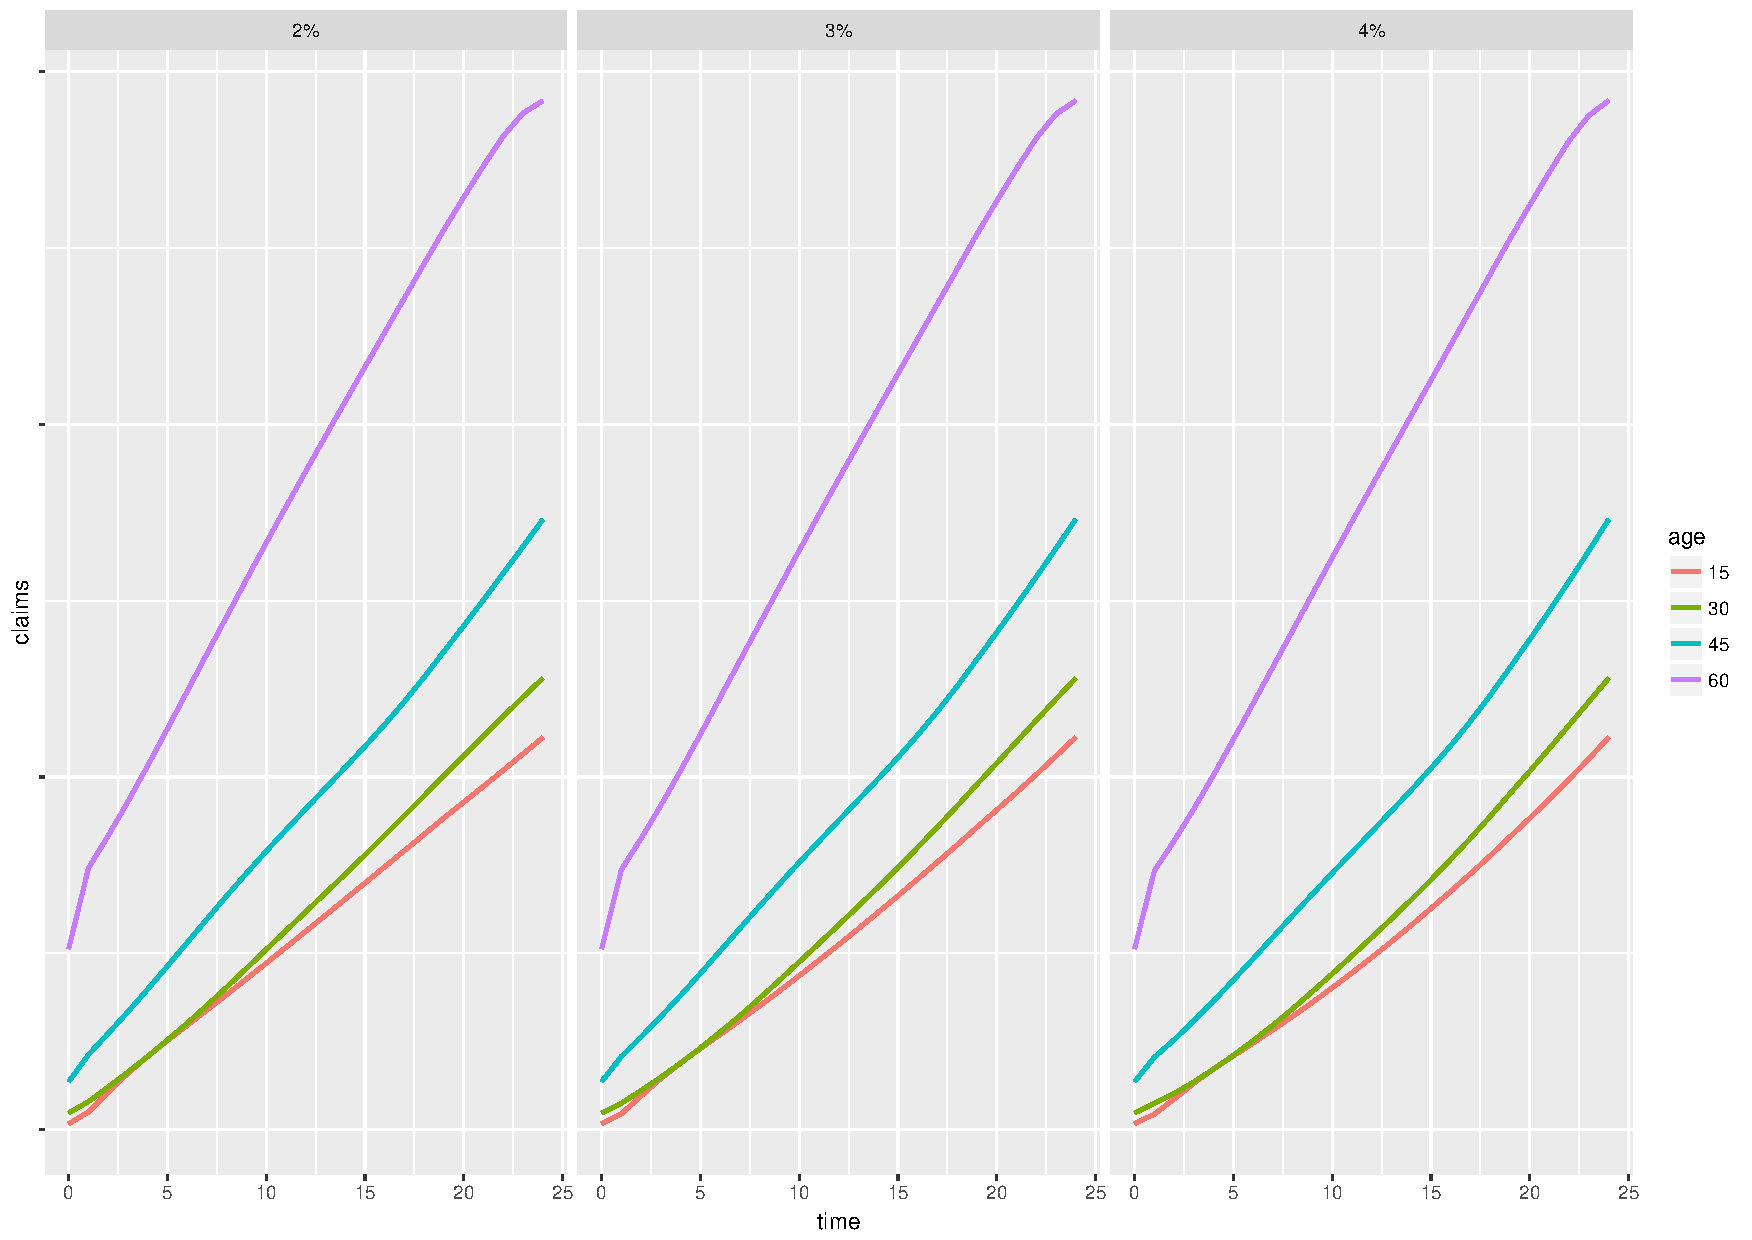
\includegraphics[width=0.9\textwidth]{figures/chapter_sensitivities/sensitivity_age_claims}
	\caption{Yearly cash flow for claims depending on the age and the technical interest rate.}
	\label{fig:sensitivity_age_claims}
	
	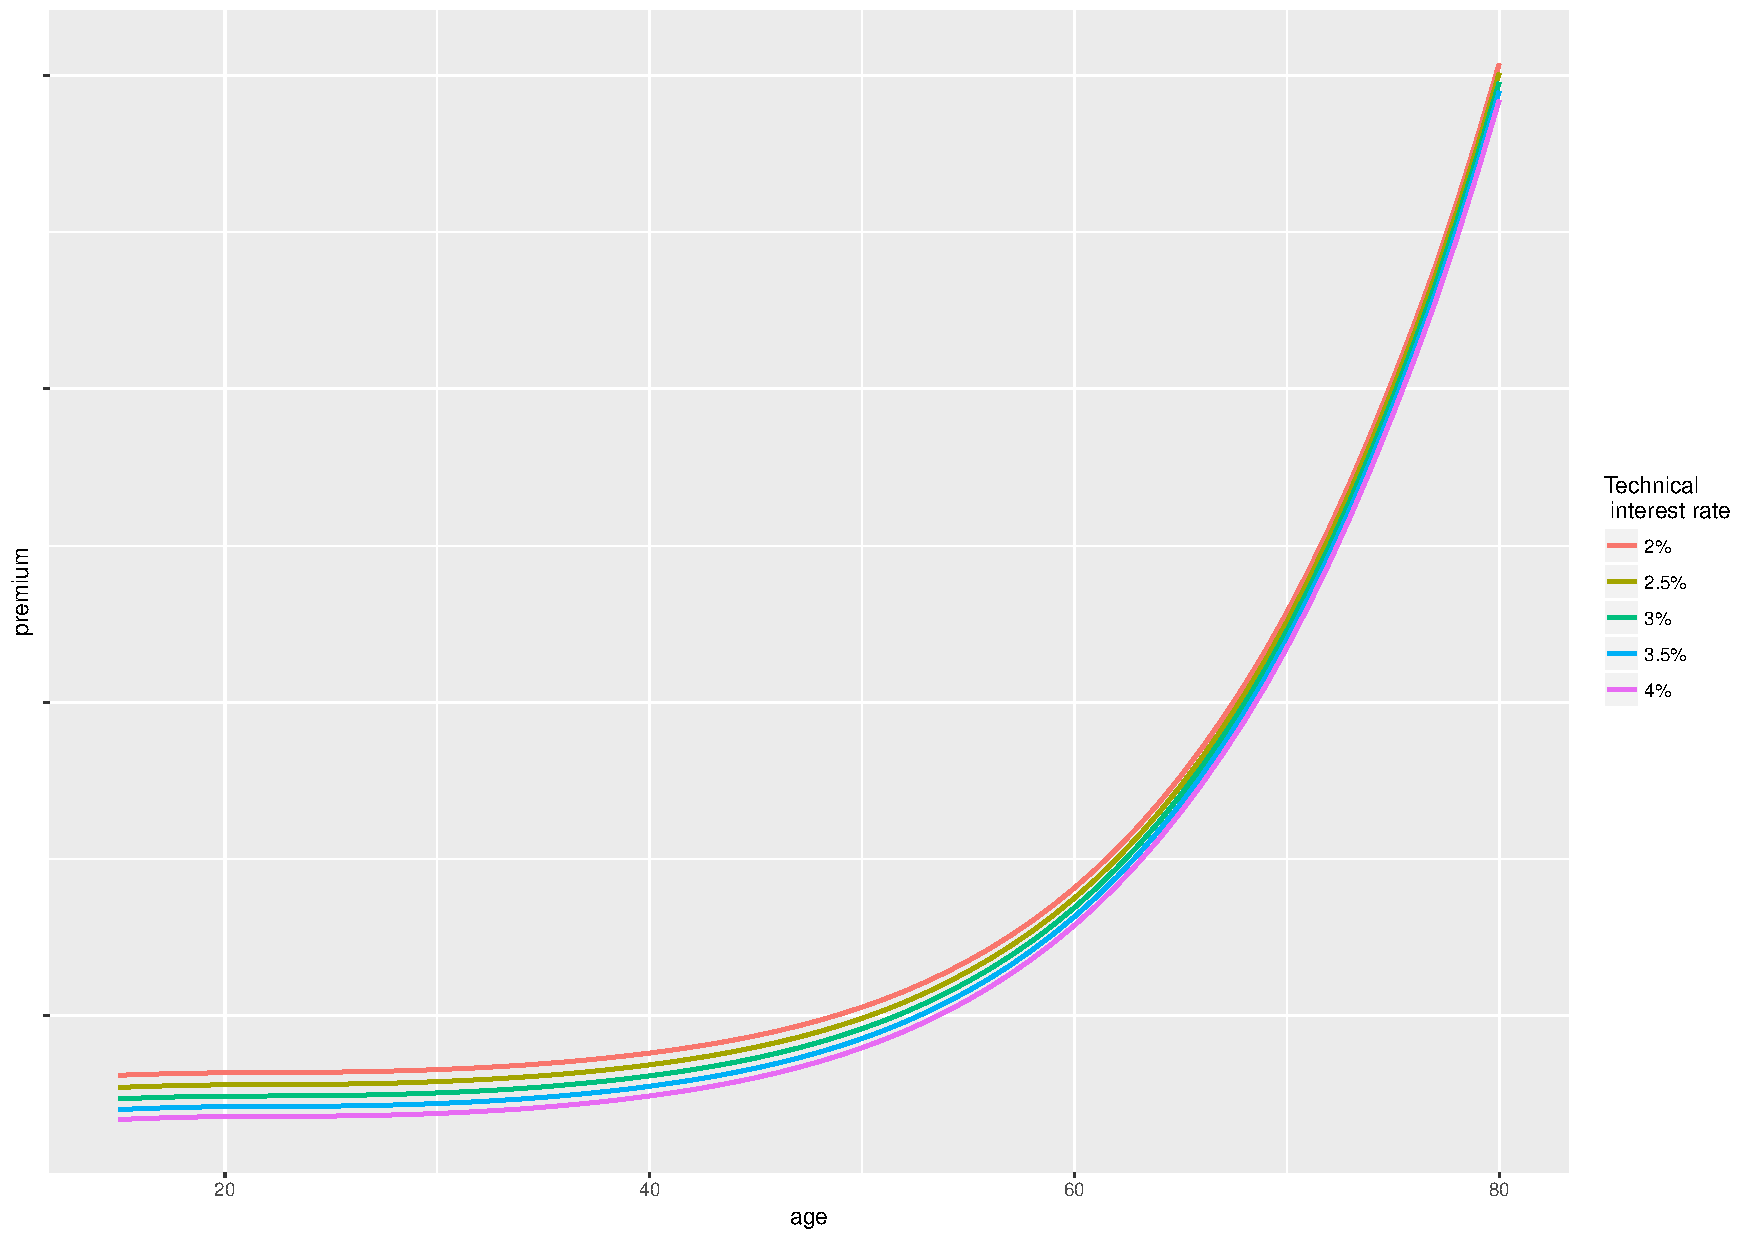
\includegraphics[width=0.9\textwidth]{figures/chapter_sensitivities/sensitivity_age_premium}
	\caption{Premiums depending on the age and the technical interest rate.}
	\label{fig:sensitivity_age_premium}
\end{figure}


\begin{figure}
	\centering
	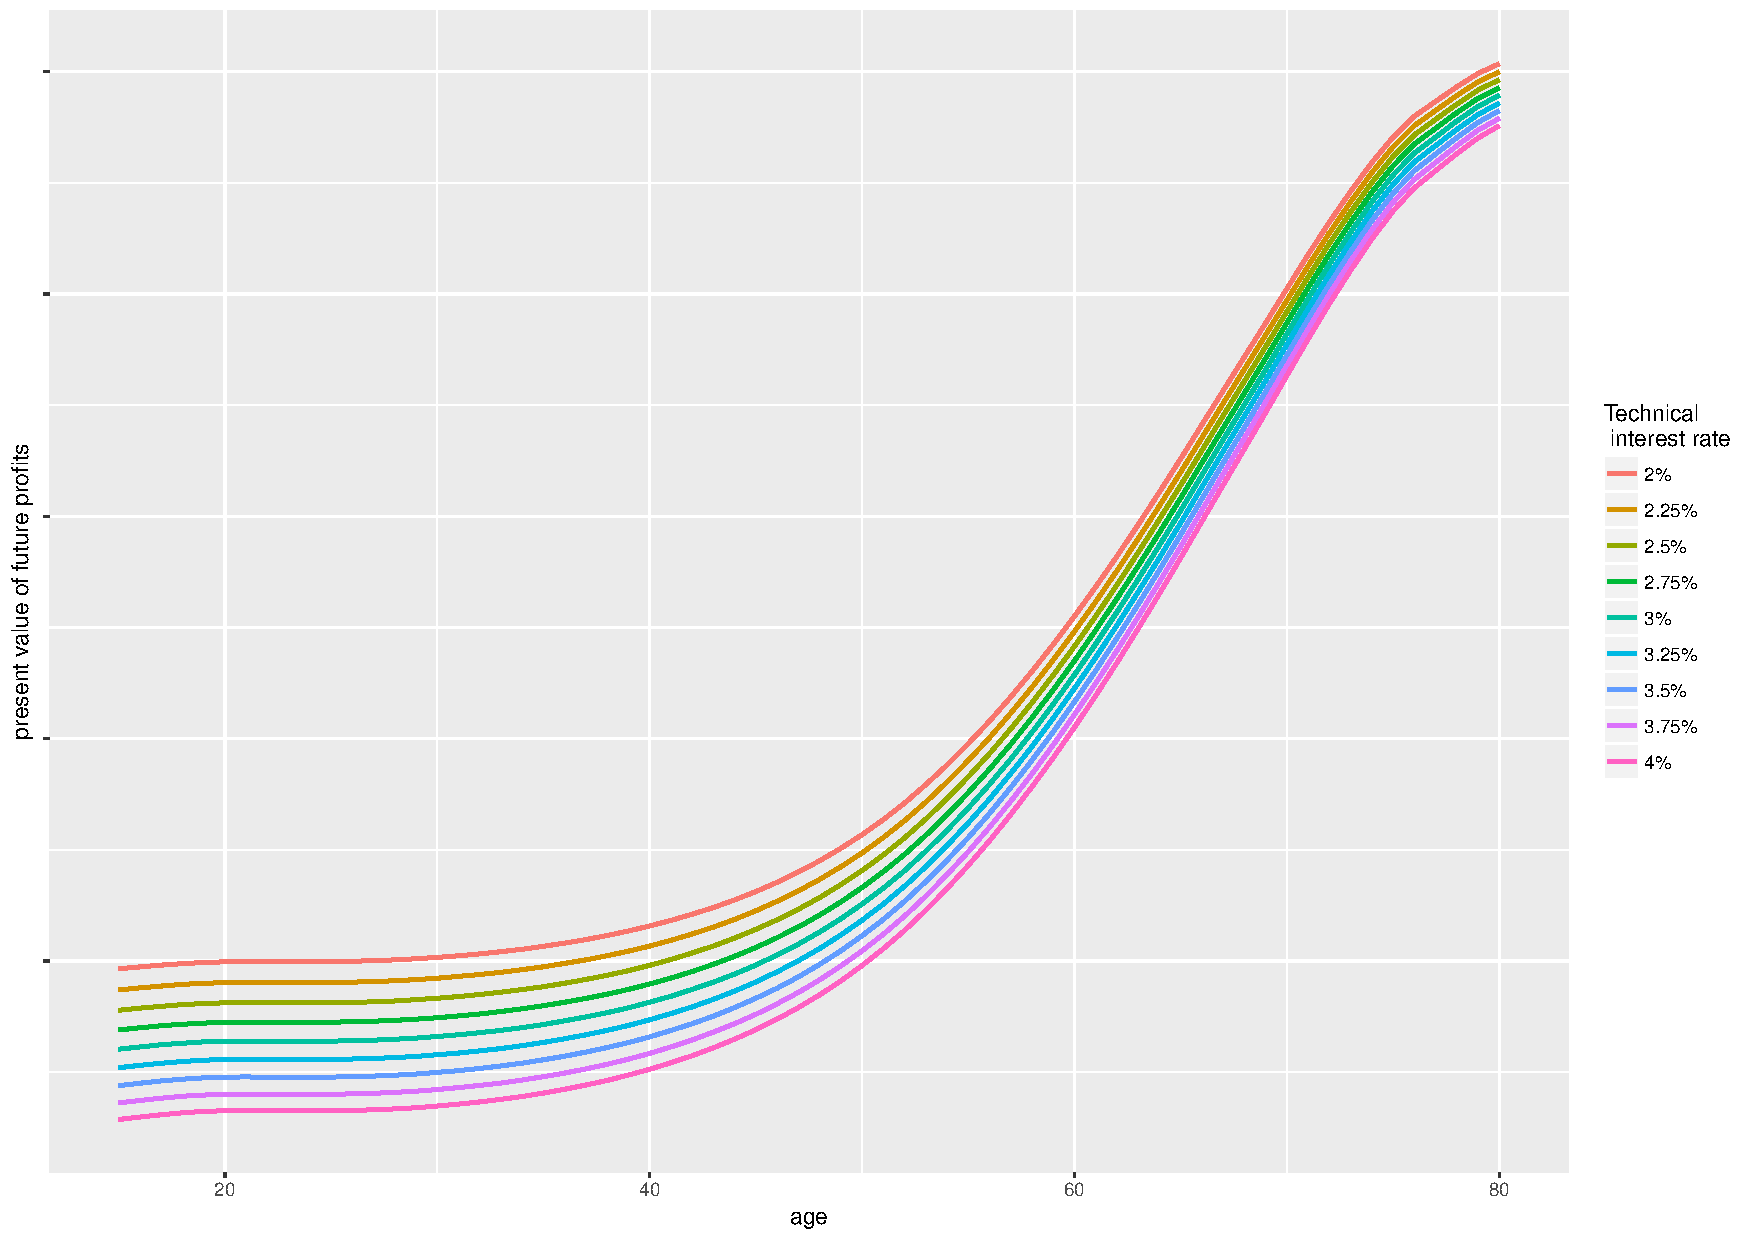
\includegraphics[width=0.9\textwidth]{figures/chapter_sensitivities/sensitivity_age_pvfp}
	\caption{Present value of future profits at time 0 depending on the age and the technical interest rate.}
	\label{fig:sensitivity_age_pvfp}

	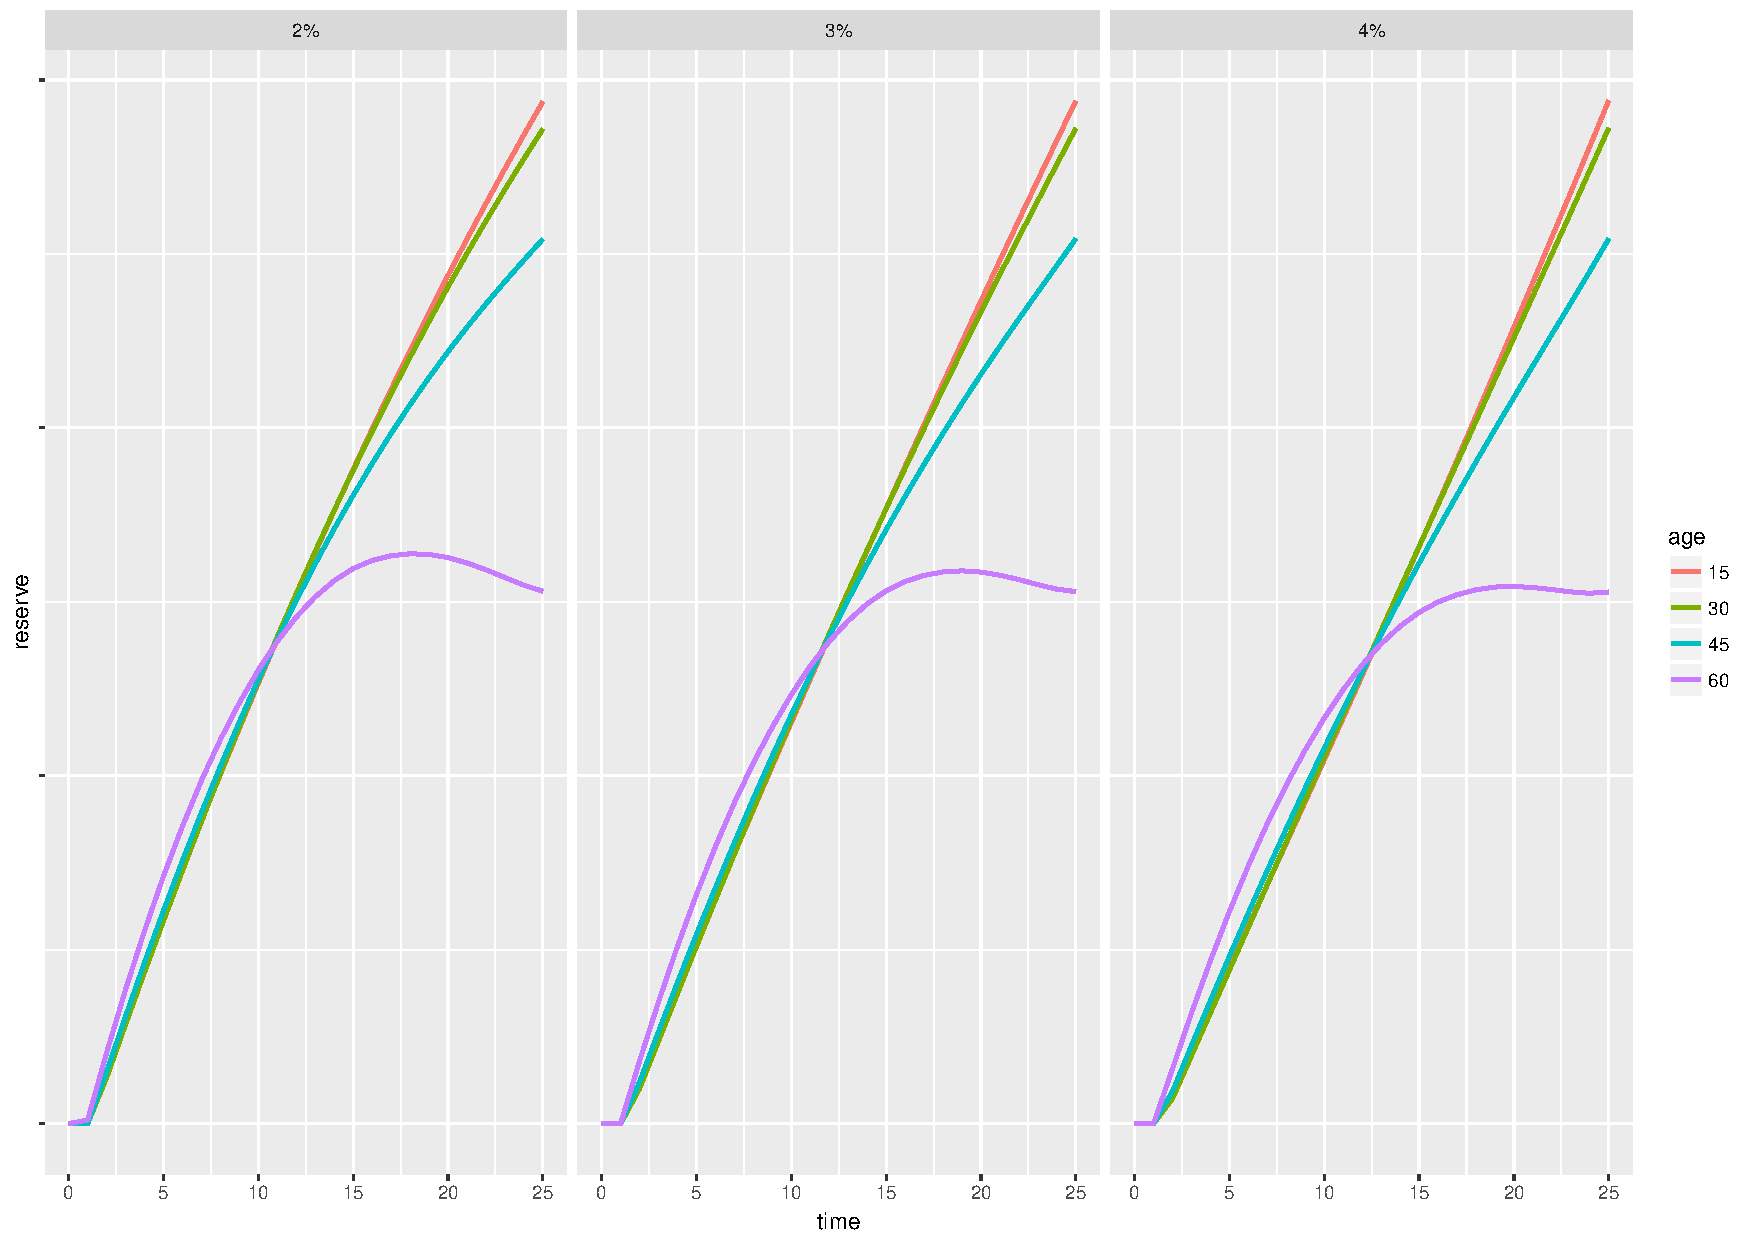
\includegraphics[width=0.9\textwidth]{figures/chapter_sensitivities/sensitivity_age_reserve}
	\caption{Yearly reserve depending on the age and the technical interest rate.}
	\label{fig:sensitivity_age_reserve}
\end{figure}


\section{Technical interest rate}
\label{sec:technical_interest_rate} 
The technical interest rate is one of the key assumptions in the life insurance business. It determines the factor by which the reserve and the savings premium increases during the contract period. After the contract has been concluded the technical interest rate is fixed and can't be changed by the insurance company. The maximum technical interest rate has been reduced dramatically by the Financial Market Authority in recent years from 4\% to 0.5\% as shown in table \ref{tab:interest_rates}.  The regulation of this upper bound is also relevant as it is often related to the minimum interest rate guaranteed to the policy holder. It is obvious that the higher the  technical interest rate, the higher the guaranteed benefit or the lower the premium will be. When the grouping algorithm forces policies from different product generations with same payout characteristics but different technical interest rates to be grouped together one important thing to be aware of are sensitivities. Another important aspect which need to be taken care of when policies with different technical interest rates are grouped together is the one of consistent management rules.  Take for example policy 1 with a technical interest rate of 2\% and a bonus rate of 2\% and policy 2 with a technical interest rate of 4\% and a bonus rate of 0\%. Lets assume that the two policies are similar and the grouped policy has a technical interest rate of 3\% and a bonus rate of 1\%. The total interest rate then is the same for the grouped and the ungrouped policies. Assume that the bonus rate is reduced by 1\% caused by a management decision. Then policy 1 has only a bonus rate of 1\% and policy 2 doesn't change at all, but the grouped policy has now a bonus rate of 0\%. The total interest rate is not the same for the grouped and the ungrouped policies which can potentially have major impacts on the projected cash flows. When the technical interest rate increases, the present value of future profits as well as the premium will decrease as shown in figure (\ref{fig:sensitivity_age_pvfp}) and (\ref{fig:sensitivity_age_premium}) respectively. This behaviour is not surprising at all, because as the technical interest rate rises the insurance company guarantees a higher benefit and this yields ceteris paribus to a lower PVFP. The reserve and the claims are not that much affected by an increase of the technical interest rate as shown in figure (\ref{fig:sensitivity_age_claims}) and (\ref{fig:sensitivity_age_reserve}) respectively.




\section{Duration}
\label{sec:duration}
The duration $n$ of an insurance contract is next to the age and the technical interest rate another main characteristic which need to be taken care of when a grouping process is carried out. In figure (\ref{fig:sensitivity_duration_claims}) the yearly claims except the last claim, which is the maturity claim, are shown for different ages. One obvious conclusion that can be derived is that the sum of all sorts of claims except the maturity claim is getting the higher the higher the age is. Another observation that can be made is that for any given time $t$ the claims are the higher the shorter the duration gets when we keep the age fixed. This is not surprising at all, because a shorter duration goes along with a higher premium (see figure (\ref{fig:sensitivity_duration_premium})) and a higher reserve (see figure (\ref{fig:sensitivity_duration_reserve})) which yields to higher claims for every fixed t.  In figure (\ref{fig:sensitivity_duration_premium}) we see that the premium is decreasing with an exponential order when the duration is increased. The difference between the premiums for policyholders with different ages is indistinguishable small for short term contracts and is getting bigger as duration increases. In figure (\ref{fig:sensitivity_duration_pvfp}) the present  value of future profits at time 0 is plotted against the duration of the contract. We see the same effect as in figure (\ref{fig:sensitivity_age_pvfp}) where contracts with higher ages lead to a higher PVFP. The effect of the absolute difference between the first and second order mortality assumptions is getting the bigger the longer the duration is and therefore the PVFP is getting the higher the longer the duration is. In the last sensitivity chart (\ref{fig:sensitivity_duration_reserve}) the reserve is plotted against the time for different values of $x$ and $n$. We see that for every time $t$ the reserve is the higher the shorter the duration is, because a shorter duration leads, ceteris paribus, to a higher premium which then results in a higher reserve. For short term contracts up to 10 years the reserve is approximately the same across different ages and is then getting the lower the higher the age and the  longer the duration is.
\begin{figure}
	\centering
	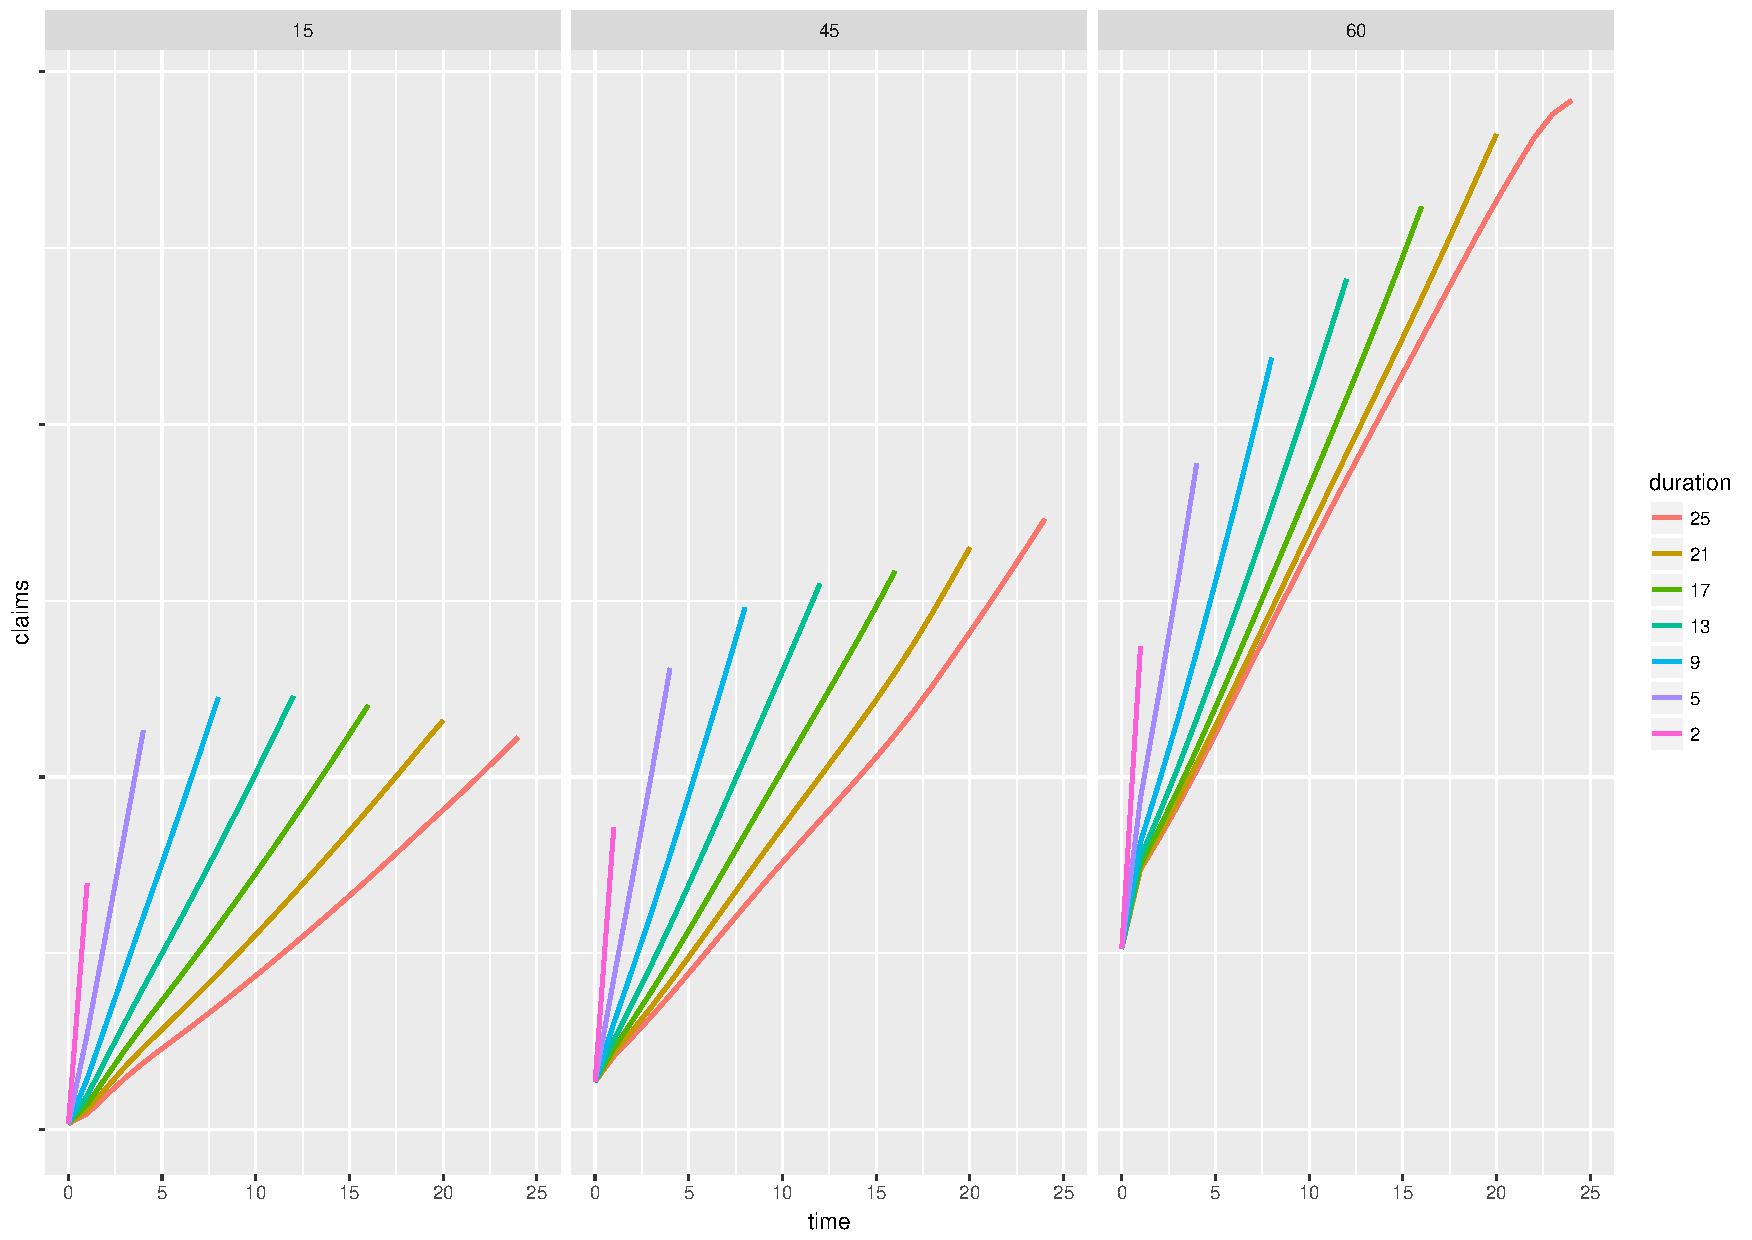
\includegraphics[width=0.9\textwidth]{figures/chapter_sensitivities/sensitivity_duration_claims}
	\caption{Yearly cash flow for claims depending on the duration and the age.}
	\label{fig:sensitivity_duration_claims}
%\end{figure}
%\begin{figure}
	\centering	
	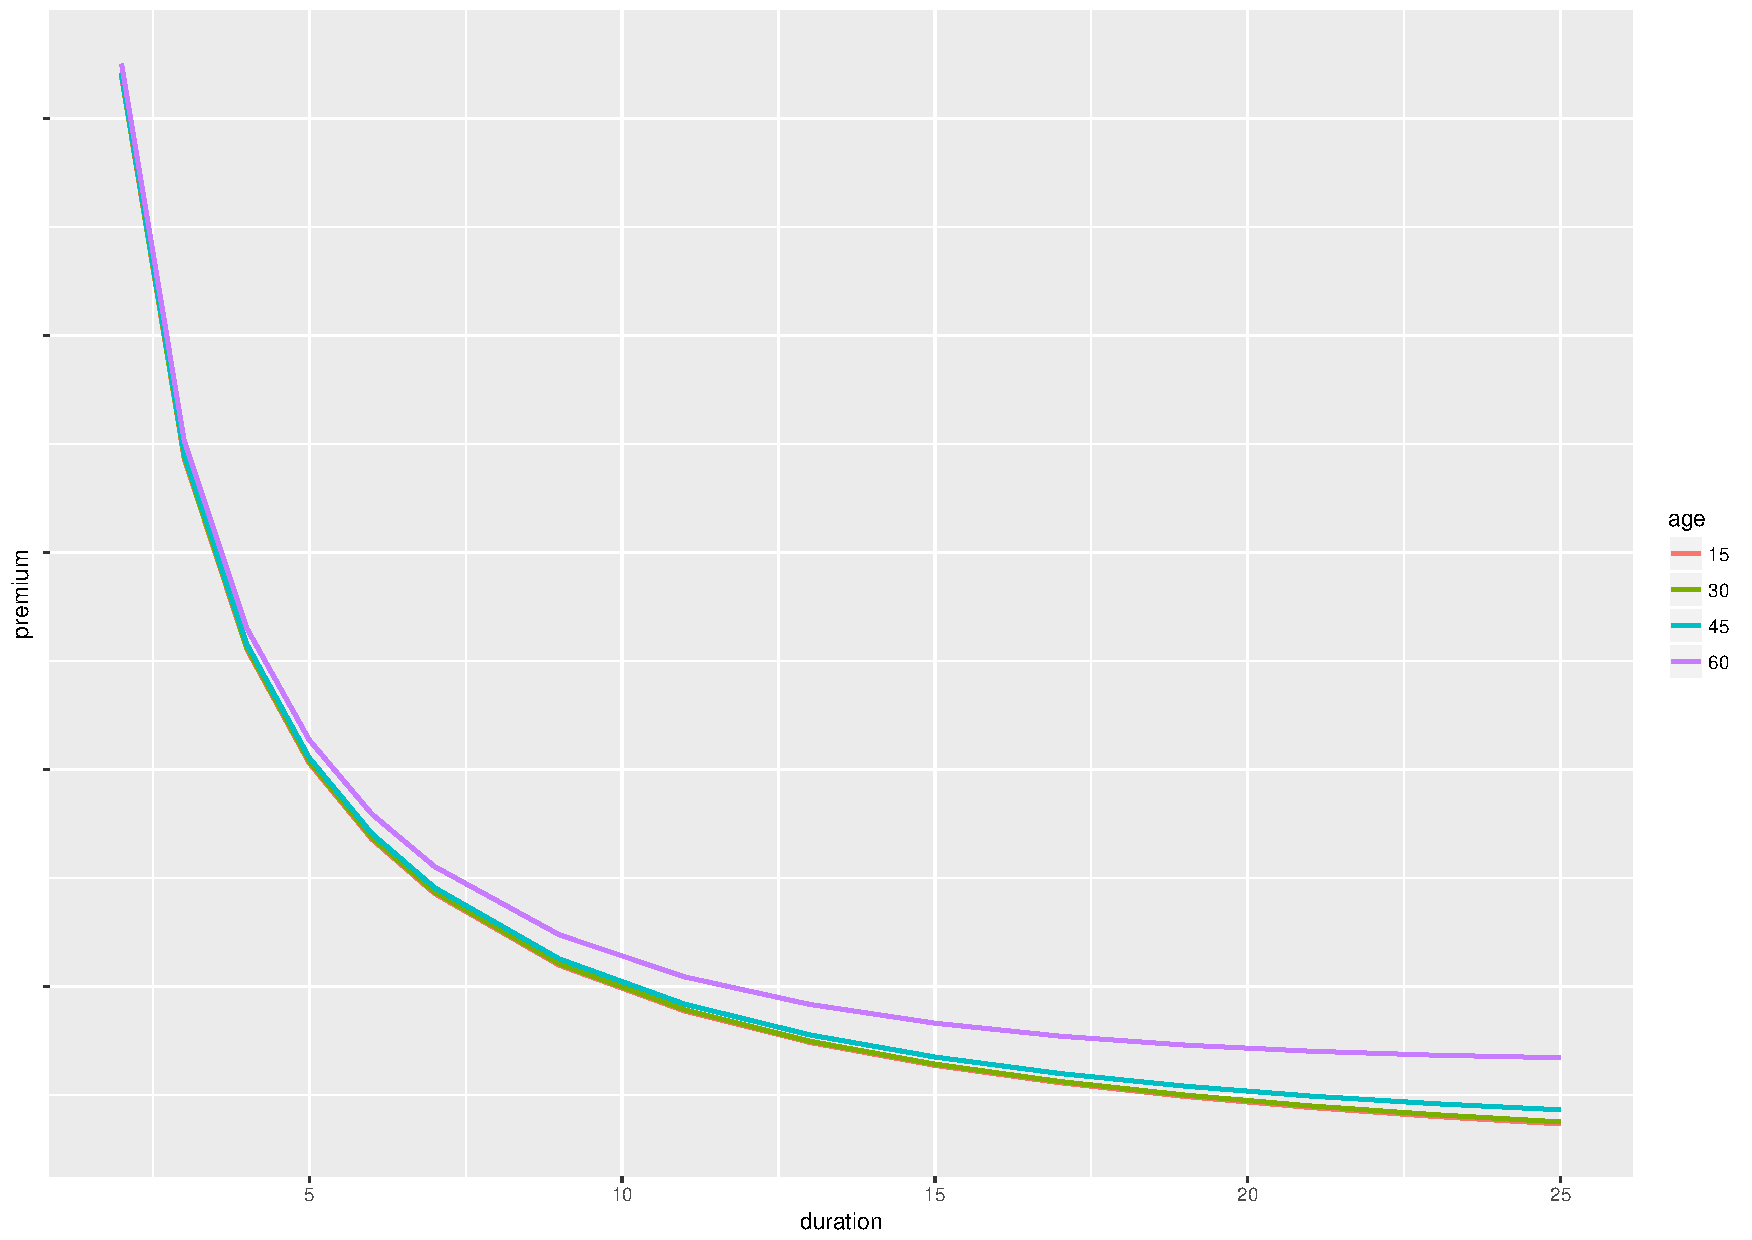
\includegraphics[width=0.9\textwidth]{figures/chapter_sensitivities/sensitivity_duration_premium}
	\caption{Premiums depending on the duration and the age}
	\label{fig:sensitivity_duration_premium}
\end{figure}



\begin{figure}
	\centering
	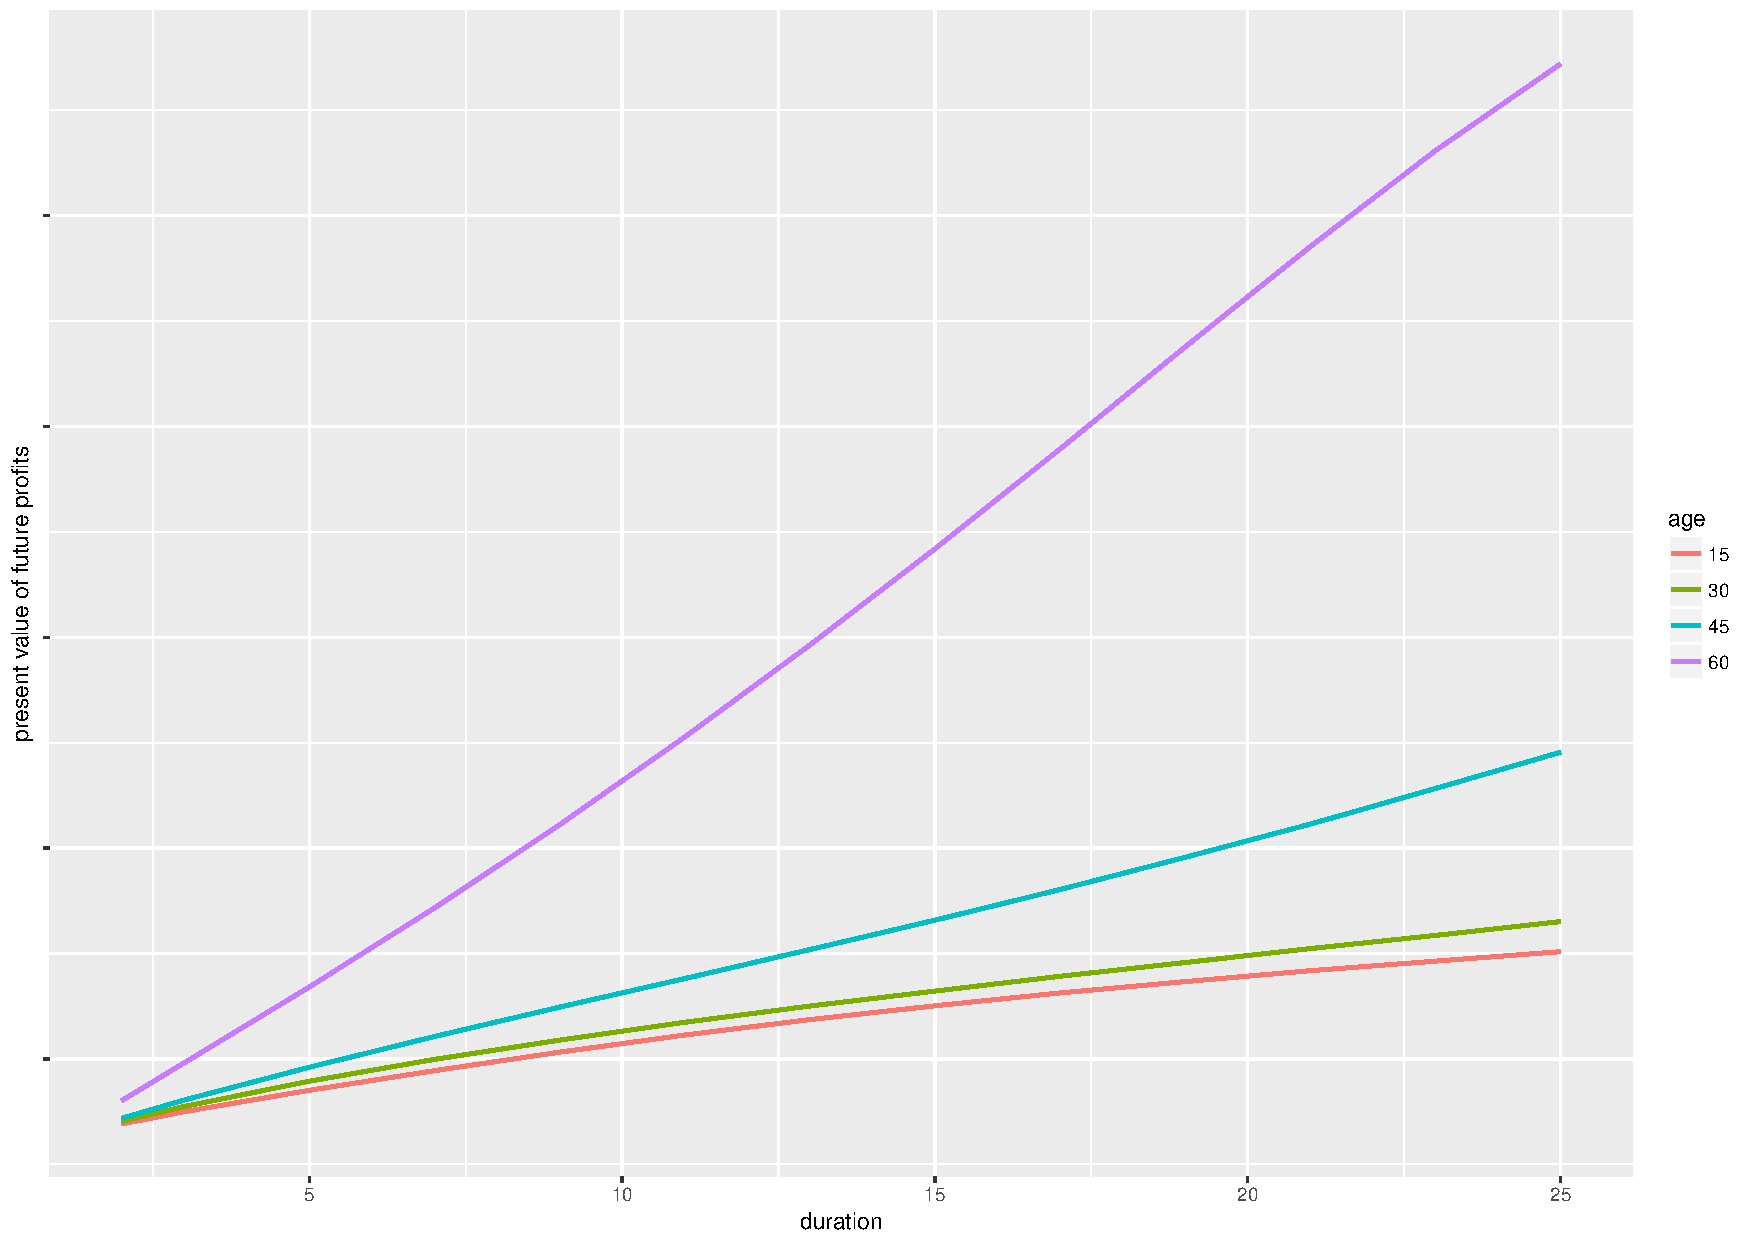
\includegraphics[width=0.9\textwidth]{figures/chapter_sensitivities/sensitivity_duration_pvfp}
	\caption{Present value of future profits at time 0 depending on the duration and the age.}
	\label{fig:sensitivity_duration_pvfp}

	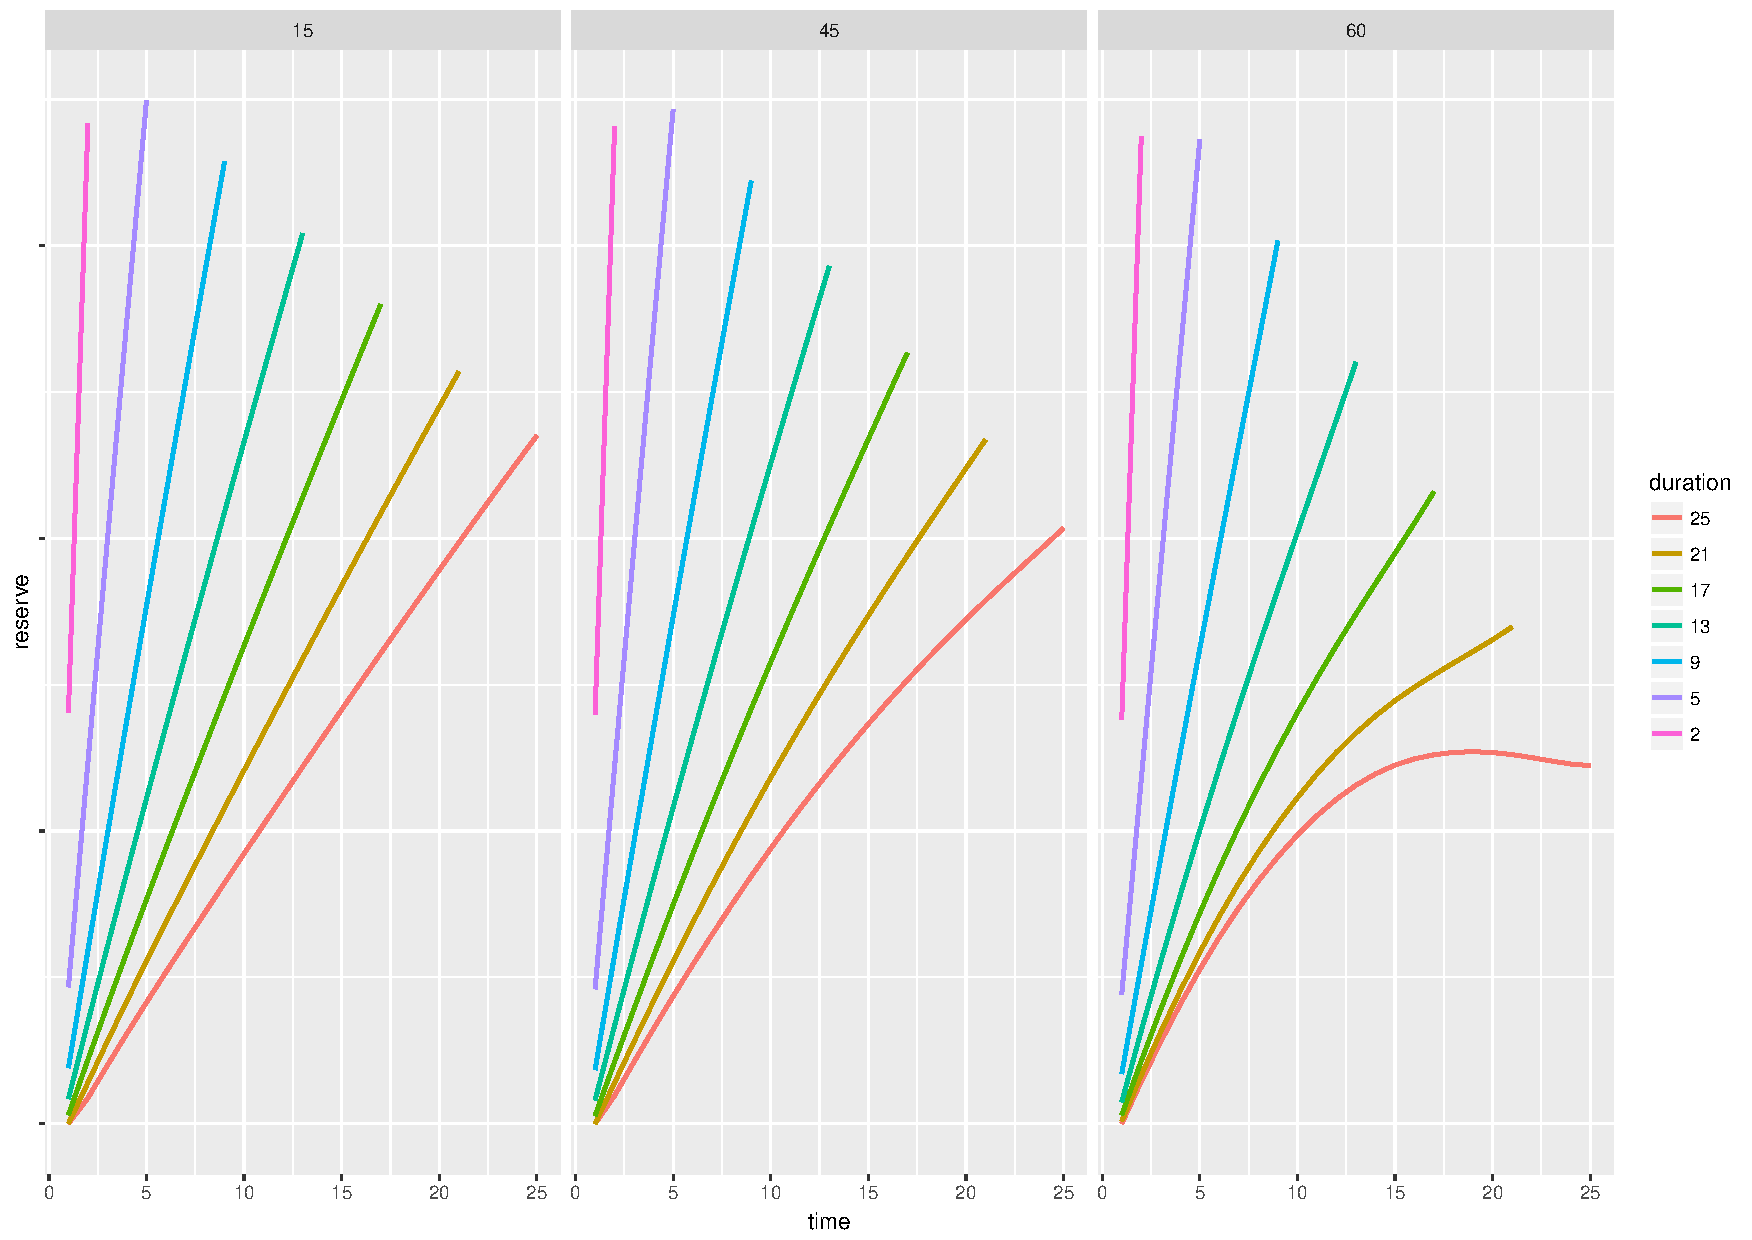
\includegraphics[width=0.9\textwidth]{figures/chapter_sensitivities/sensitivity_duration_reserve}
	\caption{Yearly reserve depending on the duration and the age.}
	\label{fig:sensitivity_duration_reserve}
\end{figure}
				%% inlcude Sensitivities
%% ========================================================================
%%							K-Means
%% ========================================================================


\chapter{$k$-means}
\label{cha:K-means}

To be able to process, summarize and understand huge amounts of data better, one is interested in methods that are able to find patterns in the data. The characteristics of these patterns then can be represented by just a few representative data points which behave like the whole data set. Given a  data set the challenge is, based on a measure of similarity, to find groups of observations which are quite similar within each group but quite different to all the other groups. If this task has to be done with unlabeled data it is referred to as unsupervised clustering (c.f.\cite{jain2010data}). One of the most widely used unsupervised clustering approaches is the $k$-means clustering. The $k$-means method is a simple approach in cluster analysis which splits a data set of $n$ $p$-dimensional observations into $k$ distinct clusters. Each observation belongs uniquely to exactly one of the $k$ clusters, where $k$ is a predefined number of clusters. Let $C=\{C_1, C_2 \dots, C_k\}$ denote the sets containing the indices of the observations  related to the clusters, then we get:
\begin{definition}
Let $X=\{x_1, ..., x_n\}$ be a data set. X is said to be partitioned into $k$ different clusters $C_1, C_2 \dots, C_k$ if
	\begin{enumerate}[label=(\roman*)] \centering
		\item $C = C_1 \cup C_2 \dots \cup C_k = \{1, \dots, n\}$

		\item $C_i \cap C_j = \emptyset \quad \forall i \neq j$
	\end{enumerate}
\end{definition}
The basic idea of the $k$-means clustering is to minimize the variation within the clusters. For this purpose some distance measure is needed in order to be able to define variation within clusters.
\begin{definition}\label{def:metric} Let X be a set, d: X$\times$X $\rightarrow~\R$ a function. Then d is called a metric (or distance) on X if for all x, y, z $\in$ X the following conditions are fulfilled: 
\begin{enumerate}[label=(\subscript{D}{\arabic*})]
	\item\label{itm:namee} $d(x,y) = 0 \Leftrightarrow x = y$ \hfill (Identity of indiscernibles)
	\item $d(x,y) = d(y,x)$  \hfill (symmetry)
	\item $d(x,z) \leq d(x,y) + d(y,z)$ \hfill (triangle inequality)
\end{enumerate}

\begin{remark}
	Given the axioms from definition \ref{def:metric} it can be shown that a non-necgativity property can be deducted e.g. $d(x,y) \geq 0 ~\forall x,y \in X$.
	\begin{equation*}
	\begin{split}
		d(x,y) + d(y,x) & \geq d(x,x) \\
		d(x,y) + d(x,y) & \geq d(x,x) \\
		2d(x,y)         & \geq 0      \\
		d(x,y)          & \geq 0      \\
	\end{split}
	\end{equation*}
	%%	\item $d(x,y) \geq 0$ \quad (non-negativity) 
\end{remark}


\begin{example}(c.f. \cite{analysis_1}) The most common used distance functions for two points $x=(x_1, ..., x_p)$ and  $y=(y_1, ..., y_p)$ in $\R^p$ are: 
	\begin{itemize}[label=$\star$]
		\item Euclidean distance:
			\begin{equation*}
				d_2(x,y) := \sqrt{\sum_{j=1}^p(x_j - y_j)^2}
			\end{equation*}
		\item Manhattan distance:
			\begin{equation*}
				d_1(x,y) := \sum_{j=1}^p|x_j - y_j|
			\end{equation*}
		\item Chebyshev (maximum) distance:
			\begin{equation*}
				d_\infty(x,y) := \max_j|x_j - y_j|
			\end{equation*}		
		\item Minkowski distance ($L^q$ distance) with q $\geq$ 1:
			\begin{equation*}
				d_p(x,y) := \bigg(\sum_{j=1}^p(x_j - y_j)^q\bigg)^{\frac{1}{q}}
			\end{equation*}	
	\end{itemize}
\end{example}

\end{definition}
Typically the Euclidean distance is used as a measure of similarity to compute the distance between the different points. By using the Euclidean metric as a measure of similarity one assumes that the clusters are spherical. 
\begin{definition}
	 Let the Euclidean metric be the measure of similarity for the data points in the data set $X=\{x_1, ..., x_n\}$ and p the dimension of the data. Then the variation within one cluster $C_l,~l=1, ..., k$ is defined as:  
	\begin{equation*}
		D(C_l) := \frac{1}{|C_l|}\sum_{j=1}^p \sum_{i,i' \in C_l} (x_{ij} - x_{i'j})^2
	\end{equation*}
\end{definition}

\begin{remark} \label{rem:average}
	For the average over one dimension in one cluster we use the short notation
	$\bar x_{lj} = \frac{1}{|C_l|} \sum_{i \in C_l} x_{ij}$.
\end{remark}

\begin{remark} \label{rem:identity}
 	The identity $\sum_{i \in C_l}(x_{ij}-\bar x_{lj})^2 = \big( \sum_{i \in C_l} x_{ij}^2 \big) - |C_l| \bar x_{lj}^2$ can be verified by simple calculus. 
\end{remark}

\begin{corollary}\label{equ:Steiner}
The variation within one cluster, $D(C_l)$ can be written as: 
	\begin{equation}
		D(C_l) =2 \sum_{i \in C_l} \sum_{j=1}^p (x_{ij}-\bar x_{lj})^2
	\end{equation}
\end{corollary}
\begin{proof}
	\begin{equation*}
	\begin{split} %% used to get only one number for all lines instead of one number per line
		D(C_l)	&= \frac{1}{|C_l|}\sum_{j=1}^p \sum_{i,i' \in C_l} (x_{ij} - x_{i'j})^2 \\
				&= \frac{1}{|C_l|}\sum_{j=1}^p \sum_{i,i' \in C_l} x_{ij}^2 - 2x_{ij} x_{i'j} + x_{i'j}^2 \\
				&= \sum_{j=1}^p \Bigg( \frac{1}{|C_l|} \sum_{i,i' \in C_l} x_{ij}^2 - 2 \frac{1}{|C_l|} \sum_{i,i' \in C_l} x_{ij} x_{i'j} + \frac{1}{|C_l|} \sum_{i,i' \in C_l} x_{i'j}^2 \Bigg) \\
				& \overset{(Remark~\ref{rem:average})}{=} \sum_{j=1}^p \Bigg( \sum_{i \in C_l} x_{ij}^2 - 2 \bar x_{lj} \sum_{i \in C_l} x_{ij} + \sum_{i' \in C_l} x_{i'j}^2 \Bigg) \\
				& \overset{(Remark~\ref{rem:average})}{=}2 \sum_{j=1}^p \Bigg( \sum_{i \in C_l} x_{ij}^2 - |C_l| \bar x_{lj}^2 \Bigg) \\
				& \overset{(Remark~\ref{rem:identity})}{=} 2 \sum_{i \in C_l} \sum_{j=1}^p (x_{ij}-\bar x_{lj})^2
	\end{split}
	\end{equation*}
\end{proof}

The approach of $k$-means is to find a partitioning of the data set in such a way that the sum of the variations is minimized.

\begin{definition}[$k$-means]
Let $X = \{x_1, ..., x_n\}$ be a data set and $\{C_1, ..., C_k\}$ a partition. Then $k$-means tries to find an optimal partition $C^* = \{C_1^*, ..., C_k^*\}$ such that: 
	\begin{equation}\label{equ:K-means}
		\sum_{l=1}^k D(C_l^*) = \underset{C_1, \dots, C_k}{\text{min}} \sum_{l=1}^k D(C_l) = \underset{C_1, \dots, C_k}{\text{min}} ~2 \sum_{l=1}^k  \sum_{i \in C_l} \sum_{j=1}^p (x_{ij}- \bar x_{lj})^2
	\end{equation}
\end{definition}

When it comes to solving the optimization problem defined by formula (\ref{equ:K-means}), the computational complexity of the algorithm to be used is of high interest. Therefore computational complexity theory categorizes problems into different classes that have some defining properties, one of which is called NP-hard. The definition of these classes would go beyond the scope of this work and therefore only a reference to the literature is given here e.g. \cite{np_hard_reference}. In very simplified terms one can say that there are currently no efficient algorithms for this type of problem. 


\begin{corollary}
	Solving the $k$-means problem defined in (\ref{equ:K-means}) is NP-hard.
\end{corollary}
\begin{proof}
c.f. \cite{NP_hard}
\end{proof}

Even though the problem is NP-hard it is still possible to provide algorithms which converge to a local optimum. The algorithms used for finding a local minimum work on an iterative basis   and involve just a few different steps. The $k$-means algorithms either start with an initial assignment of all observations to $k$ different clusters or with $k$ distinctly selected cluster centers. The next step is to find a new cluster center such that the variation $D(C_l)$ is minimized within each cluster. Then all data points $X = \{x_1, ..., x_n\}$ are reassigned to the cluster which is nearest and the minimization procedure is repeated until convergence. 

\begin{remark}~	
	\begin{enumerate}[label=(\roman*)]
		\item  For $k=n$, (\ref{equ:K-means}) is zero because each data point represents a cluster. 
	\end{enumerate}
\end{remark}

One possible formulation for an algorithm that converges to a local optimum is the one from Lloyd \cite{lloyd1982least} which a pseudo code is given below. Note that for algorithm \ref{alg:K-means} we have a fixed number of clusters $k$ as well as a finite set of possible partitions $k^n$. We can therefore show that the stated algorithm converges to a local minimum by minimizing (\ref{equ:Steiner}).

\begin{remark}~
	\begin{enumerate}[label=(\roman*)]
		\item For any set of observations S it holds that: 
			\begin{equation*}
				\bar x_S = \underset{x}{\text{argmin}}\sum_{i \in S} (x_i - x)^2
			\end{equation*}
			Hence, step \ref{lev:K-means_two}\ref{lev:K-means_two_a} minimizes the sum of squared deviations and therefore $D(C_l)$.
		\item Step \ref{lev:K-means_two}\ref{lev:K-means_two_b} which reassigns the observations to the new nearest centroid can only reduce the objective function.
	\end{enumerate}
\end{remark}

	
\begin{algorithm}
	\caption{$k$-means clustering \cite{Introducion_Stat_Learning} - Lloyd's algorithm}\label{alg:K-means}
\begin{algorithmic}
\\
	\begin{enumerate}
	\item Choose $k$ initial centroids randomly.
	\item  \label{lev:K-means_two}Iterate till the cluster assignments stop changing:
	\begin{enumerate}[label=\emph{\alph*})]
		\item \label{lev:K-means_two_a} For each of the $k$ clusters, compute the cluster centroid. The $i$-th cluster centroid is the vector of the $p$ parameter means for the observations in the $i$th cluster. 
		\item \label{lev:K-means_two_b}Assign each observation to the cluster whose centroid is closest in the sense of Euclidean distance. 
	\end{enumerate}
	\end{enumerate}
\end{algorithmic}
\end{algorithm}

%\break
\begin{remark}~
	\begin{enumerate}[label=(\roman*)]
		\item The $k$-means algorithm always converges and finds a local optimum which need not to be the global one.
		\item Different clustering results can be obtained when different initial cluster assignments in step 1 of algorithm \ref{alg:K-means} are chosen.
	\end{enumerate}
\end{remark}

\begin{remark}[Running Time]~
	\begin{enumerate}[label=(\roman*)]
		\item Algortihm \ref{alg:K-means} has a running time of $O(nkpi)$, with n being the number of data points, k the number of cluster, p the number of dimensions and i the number of iterations needed to converge. The only unknown variable is the number of iterations. 
		\item The trivial upper bound for the number of iterations needed is given by $O(k^n)$, because the algorithm visits every partition of points only once. 
		\item It can be shown \cite{arthur2006slow} that in the worst case scenario the running time of the algorithm is superpolynomial with a lower bound for the number of iterations of $O(2^{\Omega(\sqrt{n})})$. That means that the running time cannot be bounded above by any polynomial function.
		\item In practice, the number of iterations required is often small, which makes the algorithm appear to be linearly complex.  
	\end{enumerate}
\end{remark}

It is advisable to run the algorithm several times with different initial centroid assignments. This increases the likelihood of finding a partition that is close to the optimum and thus provides a low value for the objective function (\ref{equ:K-means}). However, the biggest challenge when using $k$-means is the estimation of the optimal number of clusters $k$. Figure (\ref{fig:cluster_centers}) shows an example with three clusters that illustrates the different clustering results when the number of $k$  increases. Panel (a) shows the raw data with three clusters ($k_{true} = 3$), each generated by an uniform distribution. Panels (b), (c) and (d) show the cluster results with $k = 2, 3 $ and $7$, respectively. If the number of clusters $k$ is smaller than the actual number of clusters in the data, then $k$-means merges clusters, while for $k$ greater than $k_{true}$, $k$-means divides well seperated clusters. Panel (b) shows a merge of the clusters at the top right, whereas panel (d) shows an artificial split of two natural clusters for $k=5$. For the grouping of similar data points and their representation by a cluster center, an underestimation of the actual number of clusters is more critical than an overestimation. If $k$ underestimates the true value of clusters ($k < k_{true}$), then it's  not possible to capture the cluster specific characteristics for the merged clusters because they are represented by only one cluster center. However, an overestimation of $k_{true}$ is not so critical because some natural clusters will be represented by two cluster centers which has a negative impact on the compression ratio but not the clustering quality. For the most crucial step of $k$-means, a comprehensive collection of methods for estimating the correct number of clusters can be found in \cite{milligan1985examination}. In the following, the `elbow' and silhouette method, two widely used graphical methods for estimating $k_{true}$, are presented and applied to the sample data set. 
\begin{figure}
	\centering
	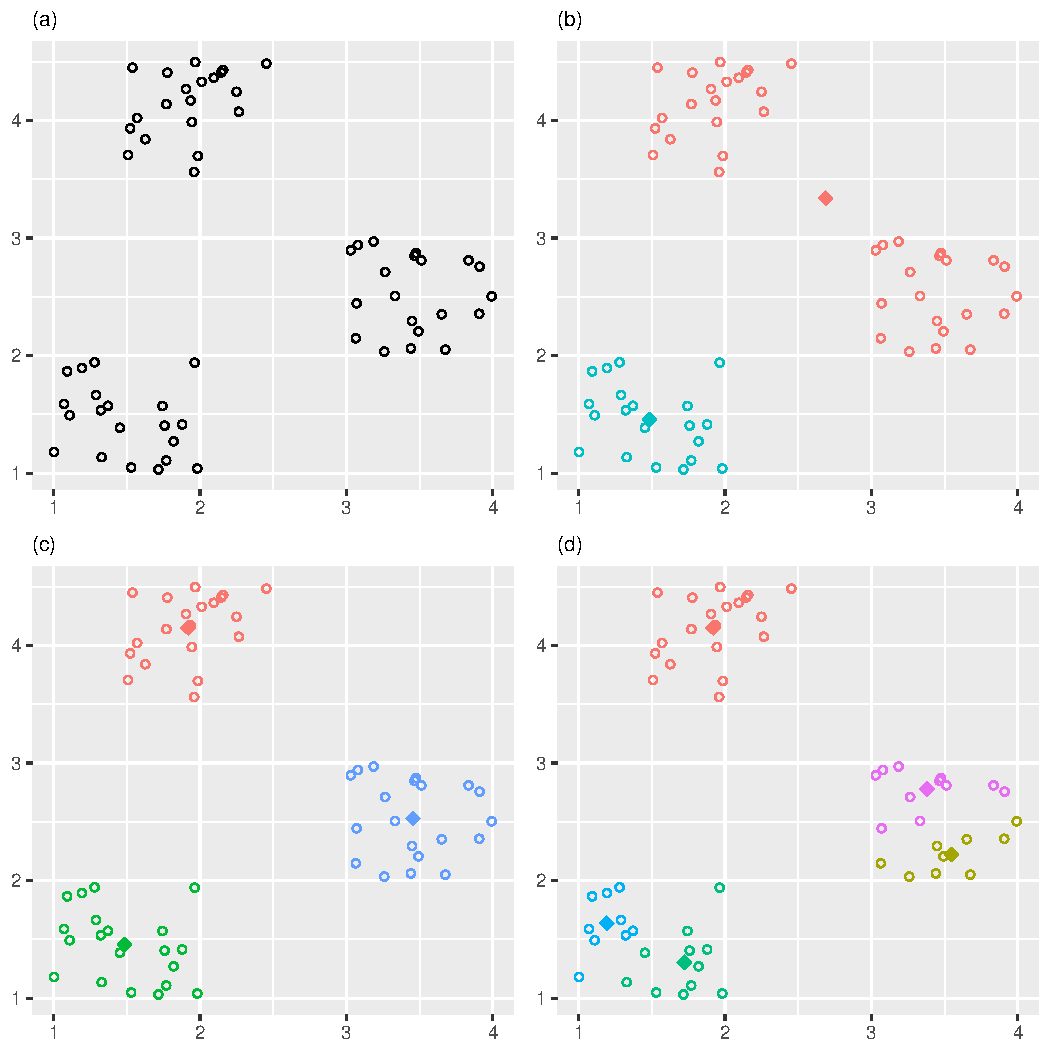
\includegraphics[width=0.8\textwidth]{figures/chapter_k_means/cluster_centers}
	\caption{Results for a three-cluster example: (a) raw data; (b) $k=2$; (c) $k=3$; (d) $k=5$}
	\label{fig:cluster_centers}
\end{figure}


\clearpage % ensure that all stuff is plotted (images)
%%%---------------------------------------------------------------------------------------------------------------------
%%%			Elbow method
%%%---------------------------------------------------------------------------------------------------------------------
\section{Elbow method - gap statistic}
Estimating $k$, the parameter that defines the number of clusters, is one of the most difficult  tasks when using k-means. While it is still possible to graphically determine the number of clusters by plotting the data in 2 or 3 dimensional spaces, other methods must be used in higher dimensions. The `elbow' method is one of the most commonly used methods in this context. 

\begin{definition}
Let $X = \{x_1, ..., x_n\}$ be a data set and k the number of clusters. Then $C=\{C_1, ..., C_k\}$ is the corresponding partition with the sum of variation within all clusters defined as: 
	\begin{equation*}
		V_k := \sum_{r=1}^k \frac{D(C_r)}{2}
	\end{equation*}
\end{definition}

 Plotting $V_k$, the sum of variation within all clusters as a measure of total error versus the number of clusters used gives a good indication for the true value of $k$. Figure \ref{fig:gap_statistics}(a) shows that the error measure $V_k$ decreases monotonically as the number of clusters increases but there seems to exist a $k$ from which the decline is clearly flattened. Such an `elbow' indicates that any additional cluster reduces the total variation $V_k$ only slightly and an appropriate number of clusters can be derived from the location of the `elbow'. In accordance with $k_{true}=3$, the `elbow' plotted in \ref{fig:gap_statistics}(a) indicates that the true number of clusters is three, because there the curve starts to flatten dramatically. Even if the sample data set consists of very well separated clusters, the example indicates that the method could also be suitable in general use cases. For a small number of tasks the graphical determination of the "elbow" is practicable, but an automated method is needed with an increasing number of clustering operations. A statistical method that formalizes this procedure of finding the `elbow' is described in \cite{tibshirani2001estimating}. The idea of the approach is to standardize $log(V_k)$ by comparing it with its expectation under an appropriate null reference distribution of the data. 
 
\begin{definition}
Let $k$ be the number of clusters and $\E_n$  the expectation with a sample size of $n$. Then the gap-statistic is defined as: 
	\begin{equation}\label{equ:gap_statistic}
		Gap_n(k) := \E_n\big[ log(V_k) \big] - log(V_k)
	\end{equation}
\end{definition}

Following the instructions in the paper and using (\ref{equ:gap_statistic}) as a measure for finding the `elbow' one takes that value of $k$ as an estimate for the number of clusters for which $Gap_n(k)$ is maximized. Taking into account the simulation error introduced by a Monte Carlo method, the proposed rule for selecting the cluster size $k$ needs to be adapted slightly. 

\begin{definition} Let $Gap(k)$ be the statistic defined above and $s_k$ the standard error (c.f. \cite{tibshirani2001estimating}). Then the rule for choosing $k$ is given by: 
	\begin{equation}\label{equ:gap_statistic_rule}
	\hat{k} := \text{smallest } k \text{ such that } Gap(k) \geq Gap(k+1) - s_{k+1}
	\end{equation}
\end{definition}

\begin{figure}
	\centering
	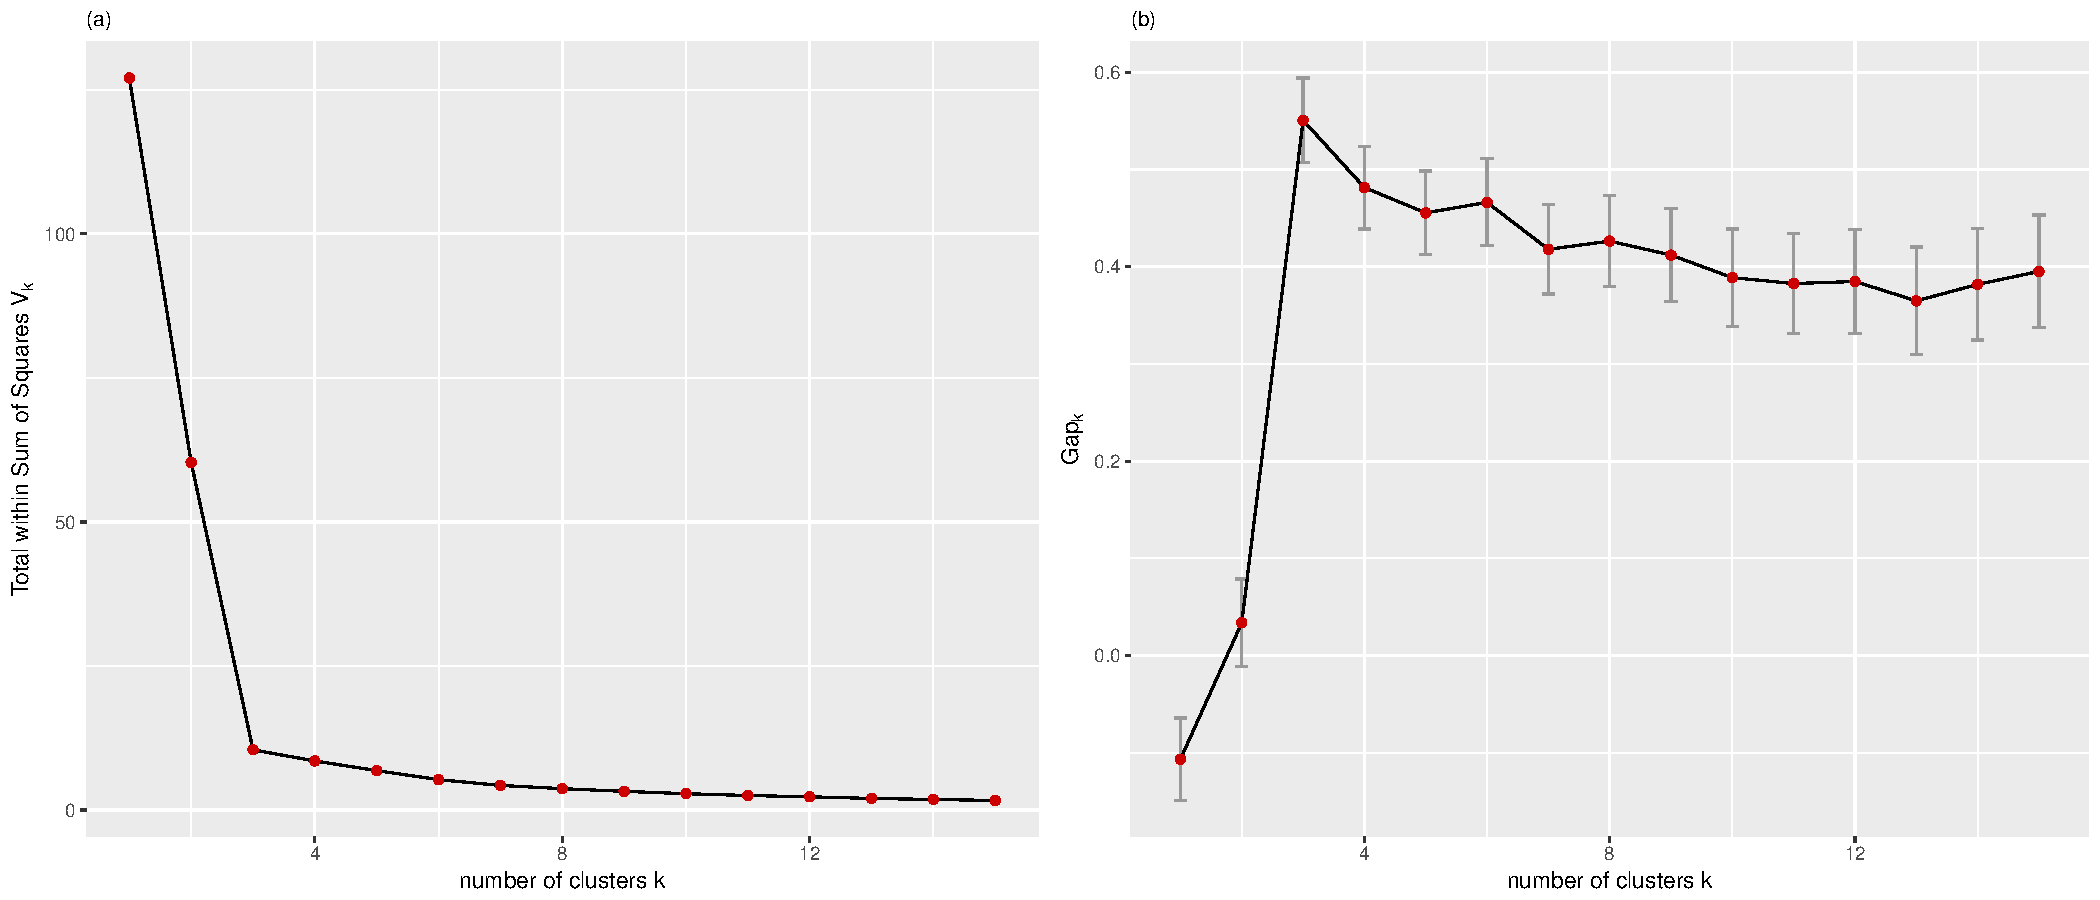
\includegraphics[width=\textwidth]{figures/chapter_k_means/gap_withinSS}
	\caption{Three-cluster example: (a) Total within Sum of Squares; (b) Gap-Statistic}
	\label{fig:gap_statistics}
\end{figure}

Figure (\ref{fig:gap_statistics})(b) shows the gap-statistic for different values of $k$ with the corresponding standard errors as a vertical bar. The application of the proposed rule (\ref{equ:gap_statistic_rule}) for selecting the number of clusters results in $\hat{k} = 3$ which corresponds exactly to the actual number of clusters in the data set. 

%%%---------------------------------------------------------------------------------------------------------------------
%%%			Silhouette method
%%%---------------------------------------------------------------------------------------------------------------------
\section{Silhouette method}\label{sec:silhouette}

Although the "elbow method" is well suited in many cases to determine the number of clusters, the resulting partitioning is not visually displayable if the dimension is larger than three. A visually appealing graphical display called silhouette plot introduced in \cite{rousseeuw1987silhouettes} tries to overcome this shortcoming in order to be able to interpret cluster results more properly. The plot shows whether a specific partitioning result reflects a cluster structure actually present in the data set or not by comparing the within dissimilarity with the between dissimilarity for every data point.

\begin{definition}[Within dissimilarity]
	Let $X=\{x_1, ..., x_n\}$ be a data set and $C=\{C_1, ..., C_k\}$ the corresponding partitioning with k cluster. Assume that the data point $x_i$ is assigned to cluster $C_A$. Then the average dissimilarity of $x_i$ to all other objects assigned to cluster $C_A$ is defined by: 
	\begin{equation*}\label{equ:dist_A}
	dist(A,i) := \frac{1}{|C_A|}\sum_{x_j \in C_A} dist(x_i, x_j)
	\end{equation*}
\end{definition}

\begin{definition}[Between dissimilarity]
	Let $X=\{x_1, ..., x_n\}$ be a data set and $C=\{C_1, ..., C_k\}$ the corresponding partitioning with k cluster. For any cluster $C_C$ different from $C_A$ the average dissimilarity of  $x_i$ to $C_C$ is given by: 
	\begin{equation*}\label{equ:dist_C}
		dist(C,i) := \frac{1}{|C_C|}\sum_{x_j \in C_C} dist(x_i, x_j)
	\end{equation*}
\end{definition}

\begin{definition}
	Let $X=\{x_1, ..., x_n\}$ be a data set and $C=\{C_1, ..., C_k\}$ the corresponding partitioning with k cluster. For any data point $x_i$ assigned to cluster $C_A$ the distance to the neighbor cluster is given by: 
	\begin{equation*}\label{equ:dist_B}
		dist(C,i) := \min_{C_C\neq C_A} dist(C,i)
	\end{equation*}
\end{definition}

Cluster $C_B$, which shares the smallest average dissimilarity with point $x_i$ is called the neighbor cluster of $x_i$. This neighbor is the first choice if cluster $C_A$ is removed from our analysis and we have to reassign $x_i$ to a new cluster. After computing $dist(A,i)$ and $dist(B,i)$ for every data point $x_i~i=1,...n$ we can define the silhouette $s(i)$ which is the most important part for visualize the clustering result.

\begin{definition}
Let $X=\{x_1, ..., x_n\}$ be a data set and $C=\{C_1, ..., C_k\}$ the corresponding partitioning with k cluster. For every $x_i \in X$ the silhouette $s(i)$ is defined as:
	\begin{equation*}\label{equ:silhouette_long}
	s(i) = \begin{cases}
		1-\frac{dist(A,i)}{dist(B,i)} 	& \text{ if } dist(A,i) < dist(B,i)\\
		0 					& \text{ if } dist(A,i) = dist(B,i)\\
		\frac{dist(B,i)}{dist(A,i)}-1 	& \text{ if } dist(A,i) > dist(B,i)
	\end{cases}
	\end{equation*}
\end{definition}

\begin{remark}
	We can write the silhouette $s(i)$ in a more compact form: 
	\begin{equation*}
		s(i) = \frac{dist(B,i) - dist(A,i)}{max\{ dist(A,i), dist(B,i) \}}
	\end{equation*}
\end{remark}

\begin{remark}
	For every $x_i$ it is true that $-1 \leq s(i) \leq 1$.
\end{remark}

\begin{remark}
	In order to understand which values of $s(i)$ correspond to which clustering results, it makes sense to look at values at the boundaries. 
	\begin{itemize}[label=$\star$]
		\item $s(i) \in (1 - \epsilon, 1]$: The within dissimilarity of $x_i$ is much smaller than the minimum between dissimilarity which indicates that $x_i$ strongly belongs to cluster $C_A$.
		\item $s(i) \in (-\epsilon, + \epsilon)$: The within dissimilarity of $x_i$ is approximately the same as the minimum between dissimilarity which indicates that $x_i$ lies between cluster A and B. It is therefore not clear whether $x_i$ should be assigned to cluster A or cluster B. 
		\item $s(i) \in [-1, -1 + \epsilon)$ The minimum between dissimilarity of $x_i$ is much smaller than the within dissimilarity which indicates that $x_i$ may not be correctly clustered. In this case $x_i$ is on average much closer to cluster $B$ than to cluster $A$ which rises doubts if the cluster assignment is right. 
	\end{itemize}
\end{remark}

\begin{remark}
	If the assignment of $x_i$ is changed from Cluster A to Cluster B, $s (i)$ becomes $-s (i)$.
\end{remark}
In order to get a visually appealing overview if a clustering result is good or not all silhouettes are plotted on top of each other. Silhouettes which belong to the same cluster are plotted together and ranked in decreasing order.

\begin{figure}
	\centering
	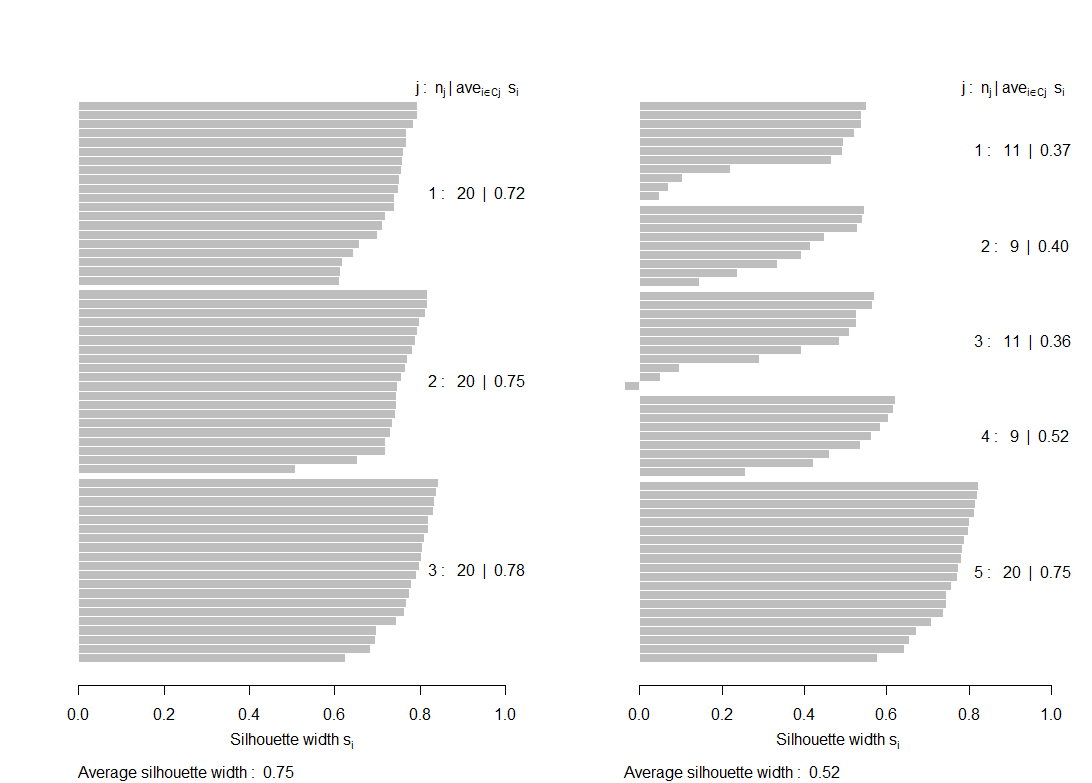
\includegraphics[width=\textwidth]{figures/chapter_k_means/silhouette}
	\caption{Left: silhouette plot for $k=3$; Right: silhouette plot for $k=5$}
	\label{fig:silhouette}
\end{figure}

Figure (\ref{fig:silhouette}) shows the silhouette plot for the sample data set with $k=3 \text{ and } 5$, respectively. Each silhouette plots shows on the right side the cluster name, the number of data points assigned to the cluster and the average silhouette width. In the right panel of figure (\ref{fig:silhouette}) cluster 1 consists of 11 data points and has a average silhouette width of $0.37$. In cluster 3 two data points have a silhouette width $s(i)$ close to zero and one data point an negative value for $s(i)$. Except for cluster 5, all other clusters include data points which have a small or even negative value for $s(i)$. At the bottom of each silhouette plot the average silhouette width for all data points is given. The silhouette plot with $k=3$ has much wider silhouettes compared to the plot with $k=5$ which is an indicator that only 3 clusters are present in the data. Similar plots for $k=2$ and $k=4$ also lead to the conclusion that the data consists of 3 natural clusters. 

\begin{remark}
A high average cluster silhouette width indicates that the cluster is well separated from other clusters and is not split up artificially. 
\end{remark}
\begin{remark}
Even though the clustering with $k=5$ is good (see figure \ref{fig:cluster_centers} (d)) the silhouette coefficient penalizes artificial splits of clusters quite heavily. 
\end{remark}

%%%---------------------------------------------------------------------------------------------------------------------
%%%			Curse of dimensionality
%%%---------------------------------------------------------------------------------------------------------------------
\section{Curse of dimensionality}
The `curse of dimensionality' is a term introduced by Richard Bellman \cite{bellman1961adaptive} to describe the rapid increase in volume and therefore the intractability of algorithms, when adding more dimensions of data to a mathematical space. Nowadays there are many different phenomenons referred to when talking about the curse of dimensionality but in the subsequent the focus is on distance functions as a measure of similarity. To get a better understanding on the issue a simple example is given that helps to illustrate the problem.

\begin{example}\label{ex:curse_of_dimensionality}~
	\begin{enumerate}[label=(\roman*)]
		\item Imagine a line segment of length 1 and 10 data points which should represent the line. To capture the whole line segment one would distribute the points uniformly across the line. Therefore the line would be divided into 10 segments with length $\frac{1}{10}$ and the points are centered within these segments.
		\item By adding one dimension the line segment becomes a square segment with edge length 1. In order to represent the `same' space with a data point as in the one-dimensional case, the square would have to be divided into 100 smaller squares with an edge length of $\frac{1}{10}$ each. In the center of each of those square segments one data point is needed as a representative. A total of 100 data points are required to represent the square segment as exactly as the line segment. 
		\item By adding another dimension the square segment becomes a cube and 1000 points are needed. 
	\end{enumerate}
\end{example}

Example \ref{ex:curse_of_dimensionality} illustrates that as the number of dimensions increases the number of data points rises exponentially in order to represent the whole space properly. Thinking of insurance data, one can have data points with various numbers of dimensions ranging from just a few to several hundreds dimensions. Considering the fact that the cash flow projections of grouped policies should coincide over a 60 year horizon, it is easy to see that only 5 of these cash flow characteristics result in data points with a dimension of 300. Of course, it is not advisable to include all cash flow variables in the grouping process over a period of 60 years, but it is much more difficult to find only those variables that are relevant for a major part of the results. For this reason, in practice more variables are often used than would actually be necessary. Another unintuitive fact one needs to be aware of is that the volume of a hypersphere inscribed into a hypercube is getting relatively smaller as the dimension increases. 

\begin{corollary}\label{cor:volume}
Let a hypersphere with radius $r$ and dimension $d$ be inscribed into a hypercube with edges of length $2r$. Then we get for the proportion of the volumes:
	\begin{equation*}
		\frac{V_{Sphere}}{V_{Cube}} =\frac{r^d\frac{\pi^{\frac{d}{2}}}{\Gamma(\frac{d}{2}+1)}}{(2r)^d} =\frac{\pi^{\frac{d}{2}}}{2^d\Gamma(\frac{d}{2}+1)} \rightarrow 0 \text{ as } d \rightarrow \infty
	\end{equation*}
\end{corollary}

\begin{remark}
Corollary \ref{cor:volume}  says that as dimension $d$ increases, more and more volume of the hypercube is outside the hypersphere. This means that under a uniform distribution most of the data points are located far from the center and thus close to an edge in a certain sense. 
\end{remark}

\begin{remark}
Some other examples why intuition fails in high dimensions are given in paragraph 6 of \cite{domingos2012few}.
\end{remark}

Not only do the data points move closer to the edge as the dimension $d$ of the data space increases, but the distance between the individual data points is becoming more and more similar. It can be shown (\cite{beyer1999nearest}) that under a broad set of conditions the distance to the nearest and to the farthest data point converges as dimensionality $d$ increases. Experimental results in \cite{beyer1999nearest} show that this effect can occur even for relatively low dimensional data with only 10 to 15 dimension. The fact that the distance to the farthest data point can get similar to the distance of the nearest data point makes clustering a hard job. The basic concept of $k$-means is to find, in the case of the Euclidean distance measure, spherically shaped clusters that have different characteristics. Therefore, data that is almost identical should not be clustered with a simple $k$-means algorithm without further analysis. Due to the fact that the $k$-means algorithm always returns a result even though there are no clusters in the data because all data points are somehow similar, it is very difficult to determine whether $k$-means is a suitable tool for clustering or not. Situations in which all data points are similar and no cluster structure is present in the data are indicated by a low silhouette coefficient. When using the methods described in section \ref{sec:silhouette}, a silhouette plot with low silhouette coefficients for the clusters indicates that the clusters found by the algorithm are not well separated. Single clustering attempts can easily be verified by an visual inspection of plots described above. With an automated clustering approach, which is necessary for large insurance portfolios, visual control of the individual silhouette plots is not possible in most cases. It is therefore advisable to use low-dimensional policy data sets or conduct a thorough analysis of the data to avoid situations where problems referred to as 'course of  dimensionality' occur. 







						%% inlcude K-means
%% ========================================================================
%%							NNLS
%% ========================================================================


\chapter{Non-negative least squares (NNLS)}
\label{cha:NNLS}

Another way to find a grouped portfolio that minimizes the deviation defined in formula (\ref{eq:objective_function}) is to solve the problem using mathematical optimization methods. The goal is to find a subset of the portfolio and scale it in way so that the square deviation becomes minimal. Of course, this approach must ensure that scaling is only possible in the positive direction. This means that it makes no sense to have a negative policy in the grouped portfolio, because it cannot be defined, not to mention explained logically. 

\begin{definition}[Non-negative least squares]\label{def:NNLS}
	Let $P \subset \V$ be a portfolio, $A \in \R^{m \times n}$ the matrix with the corresponding cashflows and $b \in \R^m$ the vector with the summed cashflows. Then $x \in \R^n$, the vector of scaling, should be optimized such that:  
	\begin{equation}\label{eq:NNLS}
		\begin{aligned}
			\argmin_x \lVert Ax -b \rVert_2^2 \\
			\text{subject to } x \geq 0
		\end{aligned}
	\end{equation}
\end{definition}

\begin{remark}
	\leavevmode % needed for items to start in new line after remark.
	\makeatletter
	\@nobreaktrue
	\makeatother
	\begin{itemize}
		\item 	The entries of the vector $x$ are the so-called scaling values for the cashflows in matrix $A$. Each entry $x_i, i \in \{1,...n\}$ that is greater than zero scales to the $i$-th column of matrix $A$ where column $i$ represents the cashflows of the $i$-th policy of the portfolio.
		\item 	It should be noted that this approach optimizes cashflows, not policies. Since there is a one-to-one relationship between cashflows and policies, the scaling factors cannot only be used to scale the cashflows but also to scale the policies in order to create a grouped portfolio. 
		\item 	Scaling policies can also involve risks, as a policy that is scaled by a factor of 2 will not necessarily produce cash flows that are also increased by a factor of 2. This can be attributed to the fact that, for example, non-linearities occur due to discount effects for higher premiums in the tariff.
	\end{itemize}
\end{remark}

\begin{remark}
	The number of policies in the grouped portfolio corresponds exactly to the number of entires greater than zero in the vector $x$.
\end{remark}

One of the well known algorithms for solving the non-negative least square problem is that of Lawson and Hanson, which uses an active set method. The steps necessary for solving that problem are given in \cite{lawson}. Additionally to those parameters defined in definition \ref{def:NNLS} one also needs a real value variable $\epsilon$ as a stopping criterion.

\begin{algorithm}
	\caption{Non-negative least squares \cite{lawson}}\label{alg:NNLS}
	\begin{algorithmic}
		\\
		\begin{enumerate}
			\item Set $P = \emptyset$, $R = \{1, ..., n\}$, $x$ = $0_{n \times 1}$
			\item Compute $w = A^\top(b - Ax)$.
			\item While $R \neq \emptyset$ and $max(w) > \epsilon$
			\begin{enumerate}[label=\emph{\alph*})]
				\item Find index $j \in R$ such that $w_j = max\{w_t, t \in R\}$.
				\item Move the index $j$ from $R$ to $P$.
				\item Let $A^P$ be $A$ restricted to the variables included in $P$.
				\item Let $s$ be a vector of same length as $x$. Let $s^P$ denote the sub-vector with indexes from $P$, and let $s^R$ denote the sub-vector with indexes from $R$.
				\item Compute $s^P = ((A^P)^\top A^P)^{-1} (A^P)^\top b$
				\item Set $s^R = 0$.
				\item While $min(s^P) \leq 0$
				\begin{enumerate}
					\item Set $\alpha = min\frac{x_i}{x_i - s_i}$ for $i$ in $P$ where $s_i \leq 0$
					\item Set $x = x + \alpha(s-x)$
					\item Move from $P$ to $R$ all indices $j \in P$ for which $x_j = 0$.
					\item Compute $s^P = ((A^P)^\top A^P)^{-1} (A^P)^\top b$
					\item Set $s^R = 0$
				\end{enumerate}
				\item Set $x$ to $s$
				\item Compute $w = A^\top(b - Ax)$.
			\end{enumerate}
		\end{enumerate}
	\end{algorithmic}
\end{algorithm}

Algorithm \ref{alg:NNLS} consists, apart from the initialization, of a main loop and an inner loop. The loops are highlighted by indentations and start at step 3 and step g) respectively. If for a variable reference is made to those indices of the variable which are contained in the set $R$, then these entries are 0. All indexes that exist in the set P, by contrast, have nonzero values. If such a variable has a negative value, the algorithm either moves it to the positive value range or sets it to zero. By setting a variable to zero, the index is also shifted from the set $P$ to the set $R$. This ensures that the following condition is met at the end of the algorithm.   
\begin{align}\label{equ:final_conditions}
\begin{split}
	x_j &> 0, \quad j \in P \\
	x_j &= 0, \quad j \in R
\end{split}
\end{align}



\begin{remark}\label{rem:gradient}
	Let $f(x) = \lVert Ax -b \rVert_2^2$ be the function, then the gradient is given by: 
	\begin{equation*}
		\nabla f(x) = \nabla \lVert Ax -b \rVert_2^2 = A^\top(Ax-b)
	\end{equation*}
	
	\begin{align*}
		\nabla \lVert Ax -b \rVert_2^2	&= \nabla (Ax-b)^\top (Ax-b) \\
										&= \nabla (x^\top A^\top - b^\top)(Ax-b) \\
										&= \nabla (x^\top A^\top Ax - x^\top A^\top b - b^\top Ax + b^\top b) \\
										&= \nabla (x^\top A^\top Ax - 2x^\top A^\top b + b^\top b) \\
										&= 2 (A^\top A x - A^\top b) \\
										&= 2A^\top (Ax - b)
	\end{align*}
\end{remark}

As shown in remark \ref{rem:gradient}, step 2 of algorithm \ref{alg:NNLS} calculates the negative gradient of the ordinary least squares problem. In the next step it is checked whether the inner loop still has to be executed or not. If the index set $R$ correspond to the empty set then all indexes are already in $P$ which means that all entries of $x$ are positive (see formula (\ref{equ:final_conditions})). This case is not desirable, as no compression can be achieved. If $max(w) \leq \epsilon$ is satisfied, the gradient has no entry large enough, so that an substantial improvement can be achieved and the algorithm has reached the optimum. If one of the two conditions in step 3) is fulfilled, the main loop is executed. 

The main loop starts with searching for the index of the gradient that is not yet present in the set $P$ and has the highest value. After this index has been moved from the set $R$ to the set $P$, the solution of a restricted least square problem is calculated in step e). This least squares problem is limited to the columns of the matrix $A$ whose indices occur in the set $P$. The result is then a vector of dimension $P$ which is indicated by the notation $s^P$. To get a solution vector of the dimension $n$, the $n - \vert P \vert = \vert R \vert$ entries $s^R$ of the vector $s$ are filled with 0 - see step f). 

\begin{example}
	Based on algorithm \ref{alg:NNLS}, be $n = 15$, $P = \{2, 3, 4, 5, 7, 9\}$ and  $R = P^c = \{1, 6, 8, 10, 11, 12, 13, 14, 15\}$ then
	\begin{equation*}
		\begin{aligned}[c]	
		s = 
		\left( 
		\begin{array}{c}
		s_{1} \\
		s_{2} \\
		\vdots\\
		s_{15}\\
		\end{array}
		\right)	
		\end{aligned}
		\qquad
		\begin{aligned}[c]
		s^P = 
		\left( 
		\begin{array}{c}
		s_{2} \\
		s_{3} \\
		s_{4} \\
		s_{5} \\
		s_{7} \\
		s_{9} \\
		\end{array}
		\right)	
		\end{aligned}
		\qquad
		\begin{aligned}[c]
		s^R = 
		\left( 
		\begin{array}{c}
		s_{1} \\
		s_{6} \\
		s_{8} \\
		s_{10} \\
		\vdots \\
		s_{15} \\
		\end{array}
		\right)	
		\end{aligned}	
	\end{equation*}
\end{example}

If all components of this least square solution (i.e. $s^P$) are positive, the solution vector $x$ is overwritten with $s$ and after a new calculation of the gradient the main loop is started again. 

If there are non positive entries in the solution, the inner loop is executed. 








							%% inlcude non-negative least squares

\appendix
%% ========================================================================
%%							Introduction
%% ========================================================================


\chapter{Tables}
\label{cha:appendix_tables}

\afterpage{%
    %\clearpage% Flush earlier floats (otherwise order might not be correct)
    \begin{landscape}% Landscape page
    \begin{minipage}{\linewidth}
    \centering
    \begin{tabular}{rrrrrrrrr}
    \toprule
    \multicolumn{1}{c}{month} & \multicolumn{1}{c}{pop\_15} & \multicolumn{1}{c}{pop\_70} & \multicolumn{1}{c}{prem\_15} & \multicolumn{1}{c}{prem\_70} & \multicolumn{1}{c}{prem\_diff} & \multicolumn{1}{c}{claims\_15} & \multicolumn{1}{c}{claims\_70} & \multicolumn{1}{c}{claims\_diff} \\
    \midrule
    0     & 1     & 1     &       &       &       &       &       &  \\
    9     & 0.999834 & 0.987259 & 385.60 & 1128.40 & 742.80 & 1.70  & 130.61 & 128.91 \\
    21    & 0.977140 & 0.947577 & 379.73 & 1092.63 & 712.90 & 4.73  & 185.70 & 180.97 \\
    33    & 0.952445 & 0.905554 & 370.17 & 1045.64 & 675.47 & 10.08 & 201.42 & 191.34 \\
    45    & 0.928273 & 0.863652 & 360.80 & 998.80 & 638.00 & 15.22 & 216.81 & 201.60 \\
    57    & 0.904661 & 0.821842 & 351.64 & 952.09 & 600.45 & 19.87 & 232.12 & 212.25 \\
    69    & 0.881638 & 0.780093 & 342.69 & 905.48 & 562.79 & 24.11 & 247.29 & 223.18 \\
    %81    & 0.859199 & 0.738372 & 333.97 & 858.93 & 524.96 & 28.26 & 262.29 & 234.03 \\
    93    & 0.837332 & 0.696652 & 325.47 & 812.40 & 486.93 & 32.45 & 277.16 & 244.71 \\
    105   & 0.816021 & 0.654913 & 317.19 & 765.86 & 448.68 & 36.70 & 291.89 & 255.19 \\
    117   & 0.795253 & 0.613146 & 309.11 & 719.31 & 410.19 & 41.02 & 306.32 & 265.29 \\
    129   & 0.775013 & 0.571358 & 301.25 & 672.72 & 371.47 & 45.41 & 320.21 & 274.81 \\
    141   & 0.755288 & 0.529577 & 293.58 & 626.11 & 332.54 & 49.85 & 333.38 & 283.53 \\
    %153   & 0.736066 & 0.487855 & 286.11 & 579.53 & 293.42 & 54.35 & 345.54 & 291.19 \\
    165   & 0.717332 & 0.446430 & 278.82 & 533.03 & 254.20 & 58.90 & 354.70 & 295.80 \\
    177   & 0.699076 & 0.405693 & 271.73 & 486.94 & 215.21 & 63.50 & 359.06 & 295.56 \\
    189   & 0.681284 & 0.365984 & 264.81 & 441.73 & 176.92 & 68.15 & 359.15 & 291.01 \\
    201   & 0.663944 & 0.327583 & 258.07 & 397.76 & 139.68 & 72.83 & 355.49 & 282.66 \\
    213   & 0.647046 & 0.290722 & 251.51 & 355.31 & 103.81 & 77.54 & 348.61 & 271.07 \\
    %225   & 0.630579 & 0.255590 & 245.10 & 314.64 & 69.54 & 82.28 & 338.92 & 256.64 \\
    237   & 0.614523 & 0.222339 & 238.87 & 275.96 & 37.09 & 87.12 & 326.91 & 239.79 \\
    249   & 0.598856 & 0.191115 & 232.78 & 239.40 & 6.62  & 91.79 & 312.50 & 220.71 \\
    261   & 0.583562 & 0.162081 & 226.85 & 205.15 & -21.70 & 96.52 & 295.62 & 199.10 \\
    273   & 0.568621 & 0.135426 & 221.05 & 173.38 & -47.67 & 101.35 & 276.01 & 174.66 \\
    285   & 0.554015 & 0.111340 & 215.39 & 144.32 & -71.07 & 106.29 & 253.63 & 147.35 \\
    297   & 0.539728 & 0.089980 & 209.85 & 118.16 & -91.69 & 111.28 & 228.95 & 117.68 \\
    309   & 0.000000 & 0.000000 & 0.00  & 0.00  & 0.00  & 5983.32 & 991.18 & -4992.14 \\
    \bottomrule
    \end{tabular}%
    \captionof{table}{Yearly outputs for PVFP-sensitivity analysis.}
    \label{tab:PVFP_sensitivity}%  
    \end{minipage}
    \end{landscape}
    %\clearpage% Flush page
    }
    
test					%% inlcude appendix

The todo text 
is the text that will be shown in the todonote and in the
list of todos. The optional argument options, allows the user to customize the
appearance of the inserted todonotes. For a description of all the options see
\todo{Make a cake \ldots}
sadf
The todo text is the text that will be shown in the todonote and in the
list of todos. The optional argument options, allows the user to customize the
appearance of the inserted todonotes. For a description of all the options see
The todo text is the text that will be shown in the todonote and in the
list of todos. The optional argument options, allows the user to customize the
appearance of the inserted todonotes. For a description of all the options see
The todo text is the text that will be shown in the todonote and in the
list of todos. The optional argument options, allows the user to customize the
appearance of the inserted todonotes. For a description of all the options see
fasd
fadsf
asdf
\missingfigure{Make a sketch of the structure of a trebuchet.}

\printbibliography  %% remove, if using BibTeX instead of biblatex
\end{document}

